\section{Results}

We split our findings into the following subsections.
The basics (\ref{subsection:eval_basics}) explain and showcase the simplest base-case and what graphs we use to visualize our findings for all experiments.
Afterward (\ref{subsection:eval_image_builder}), we analyze how different variables change the image build processes.
Penultimately (\ref{subsection:eval_diff_projects}), we discuss how different ML repositories, frameworks and datasets perform in FLOps.
Lastly (\ref{subsection:eval_multicluster_hfl}), we focus on HFL and verify that our custom novel solution is sound.

\subsection{Basics} \label{subsection:eval_basics}

This subsection introduces the different plots we use to visualize all our results.
This part focuses on experiment (1).
All mentioned graphs are also available for all other experiments.
Showcasing all of them would heavily bloat this work.
Thus, we omit them.
Several additional plots are available in the appendix \ref{appendix:evaluation_plots}.
All graphs and their underlying CSV files are available in the extended OAK CLI code's evaluation folder \cite{cli_code}.


\subsubsection{CPU \& Memory}

Graph \ref{fig:eval_1_simplest_cpu_mem} shows the recorded CPU and memory utilization across a project's lifetime with stage information.
This information shows the mean of all ten evaluation runs with a 95\% confidence interval.
The colored areas represent specific project stages.
The graph unveils that the memory utilization stays relatively stable throughout a project and only slightly increases during FL training and the non-base image FL actor builds.
Note that the FL-Actors Image Build stage represents the entire image build and push process, which includes the base image and the actor images.
Deployment stages represent time frames in which components and services for the next stage are created and deployed via the FLOps manager and orchestrator, but these services/images do not yet start their workloads.
Most stages do not utilize much of the available CPU except during the FL actor deployment stage and FL training, which makes sense because this experiment uses the CPU for training.
On average, this simple base case takes 12 minutes to complete on the monolith system.

Figure \ref{fig:eval_1_simplest_cpu_boxviolin} shows a box-violin plot of the CPU utilization for different experiment stages.
The largest median CPU utilization occurs in the FL training stage.
What is remarkable is that the deployment stage for the FL actors (Aggregator Deployment in the plot) also has high CPU utilization.
Multiple services' rapid creation, deployment, and orchestration can explain this.
Both image build stages have many outliers, indicating that the build process is highly heterogeneous.

Figure \ref{fig:eval_1_simplest_memory_boxviolin} is similar to the previous plot but depicts the memory utilization per stage.
The FL training stage is the most consuming one.
All other stages are below 60\% memory utilization except for the FL actors builder and its deployment stages, which have multiple outliers that reach the high 70s.
Unlike CPU outliers, which only lead to throttling, memory outliers can lead to out-of-memory exceptions and failures.
Thus, it is vital to be aware of such behavior.

\begin{figure}[H]
    \begin{adjustwidth}{-0.2\paperwidth}{-0.2\paperwidth}
        \centering
        % 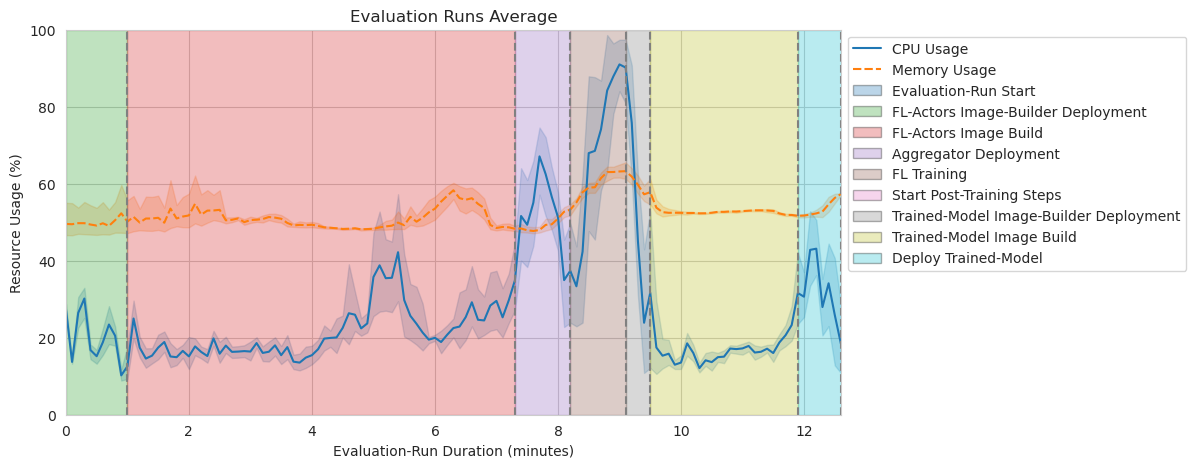
\includegraphics[width=0.95\paperwidth]{eval_1_simplest_cpu_mem.png}
        \includegraphics[width=0.95\paperwidth]{evaluations/experiment_1/cpu_mem.pdf}
        \caption{Experiment 1: CPU \& Memory Utilization}
        \label{fig:eval_1_simplest_cpu_mem}
    \end{adjustwidth}
\end{figure}

\begin{figure}[p]
    \begin{adjustwidth}{-0.2\paperwidth}{-0.2\paperwidth}
        \centering
        % 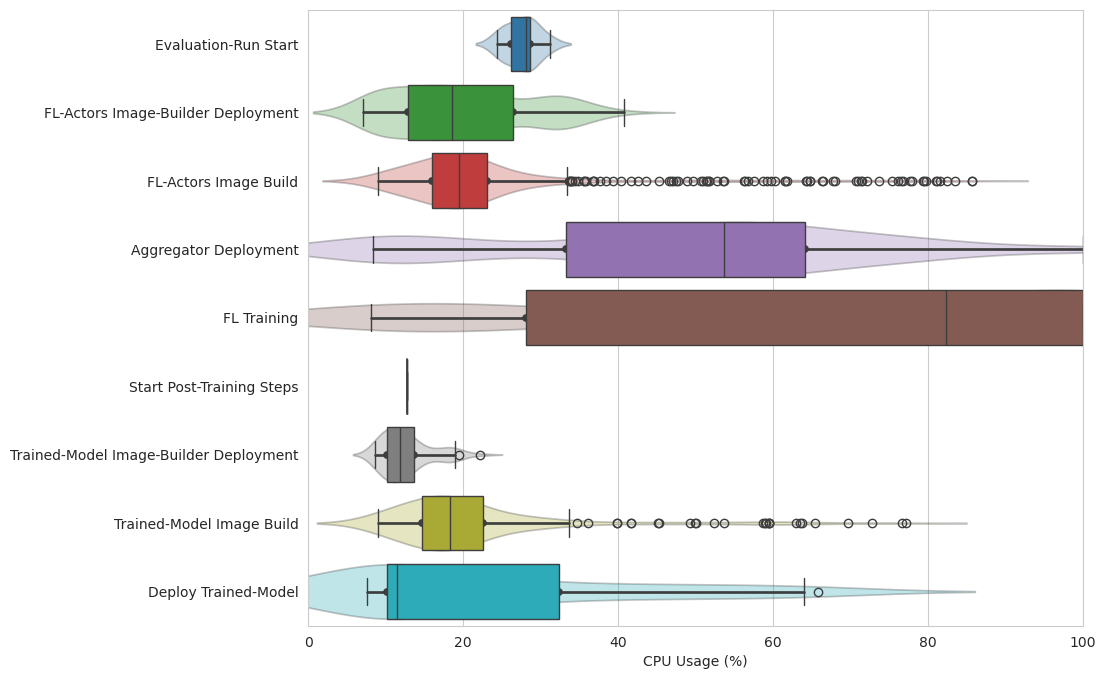
\includegraphics[width=0.70\paperwidth]{eval_1_simplest_cpu_boxviolin.png}
        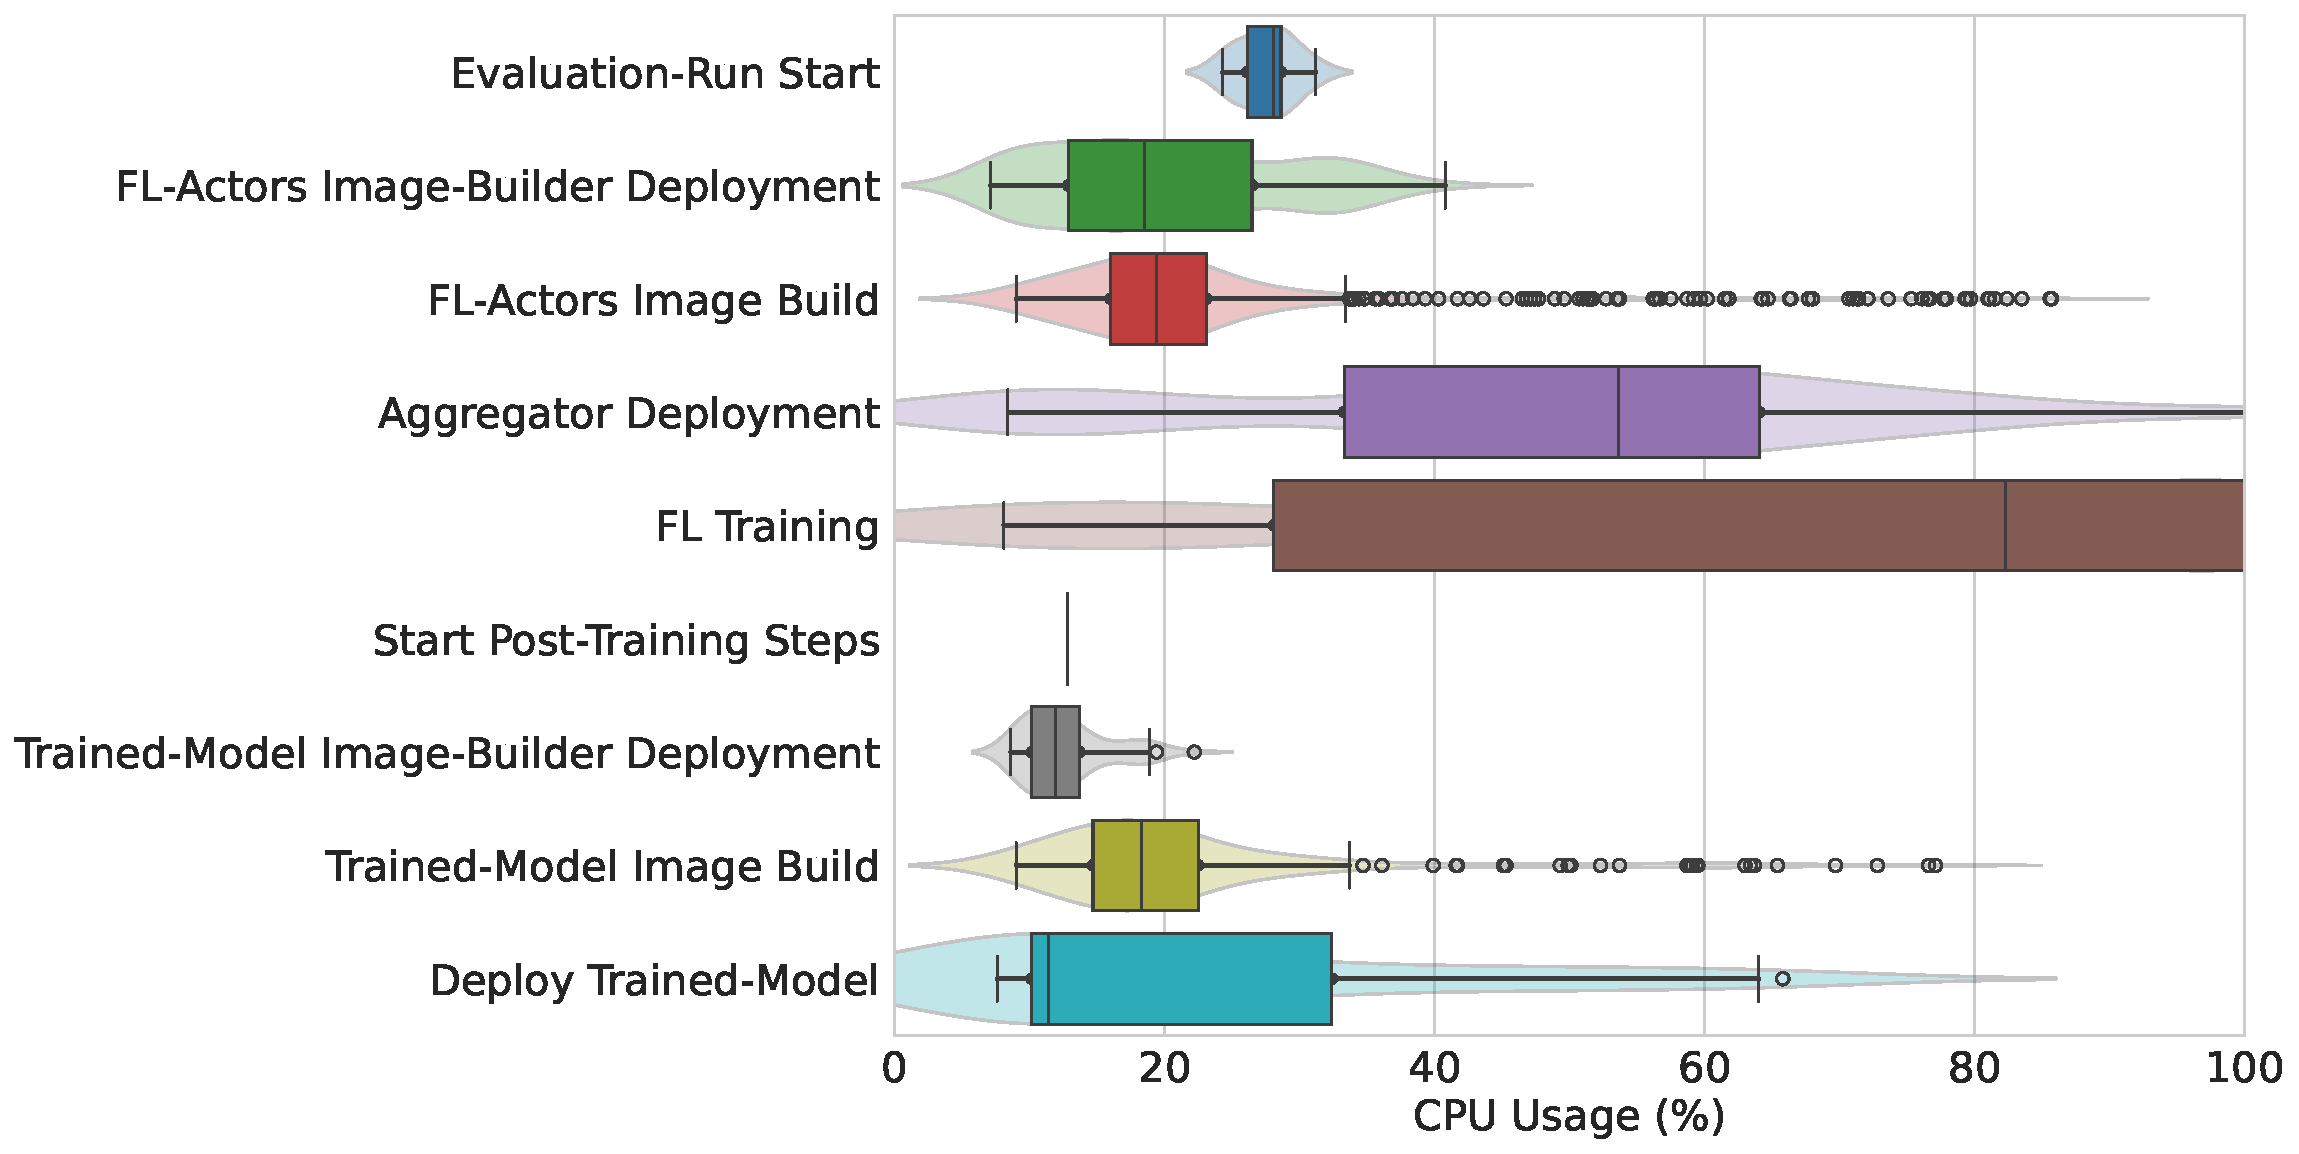
\includegraphics[width=0.85\paperwidth]{evaluations/experiment_1/cpu_by_stage.pdf}
        \caption{Experiment 1: CPU Utilization by Stage}
        \label{fig:eval_1_simplest_cpu_boxviolin}
    \end{adjustwidth}

    \begin{adjustwidth}{-0.2\paperwidth}{-0.2\paperwidth}
        \centering
        % 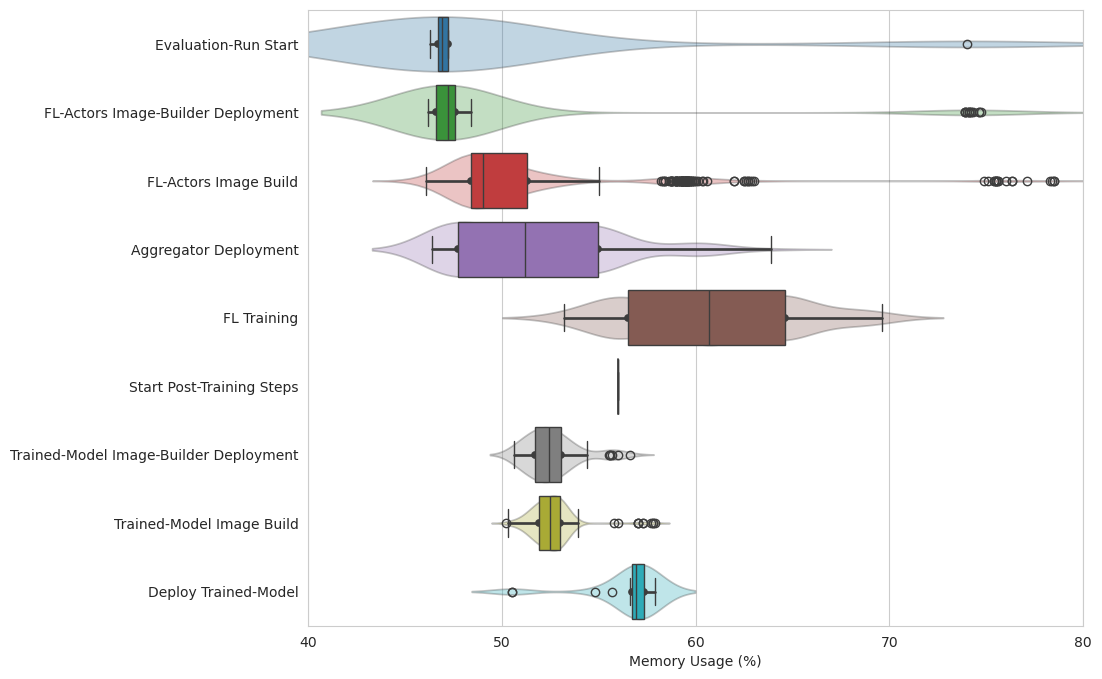
\includegraphics[width=0.70\paperwidth]{eval_1_simplest_memory_boxviolin.png}
        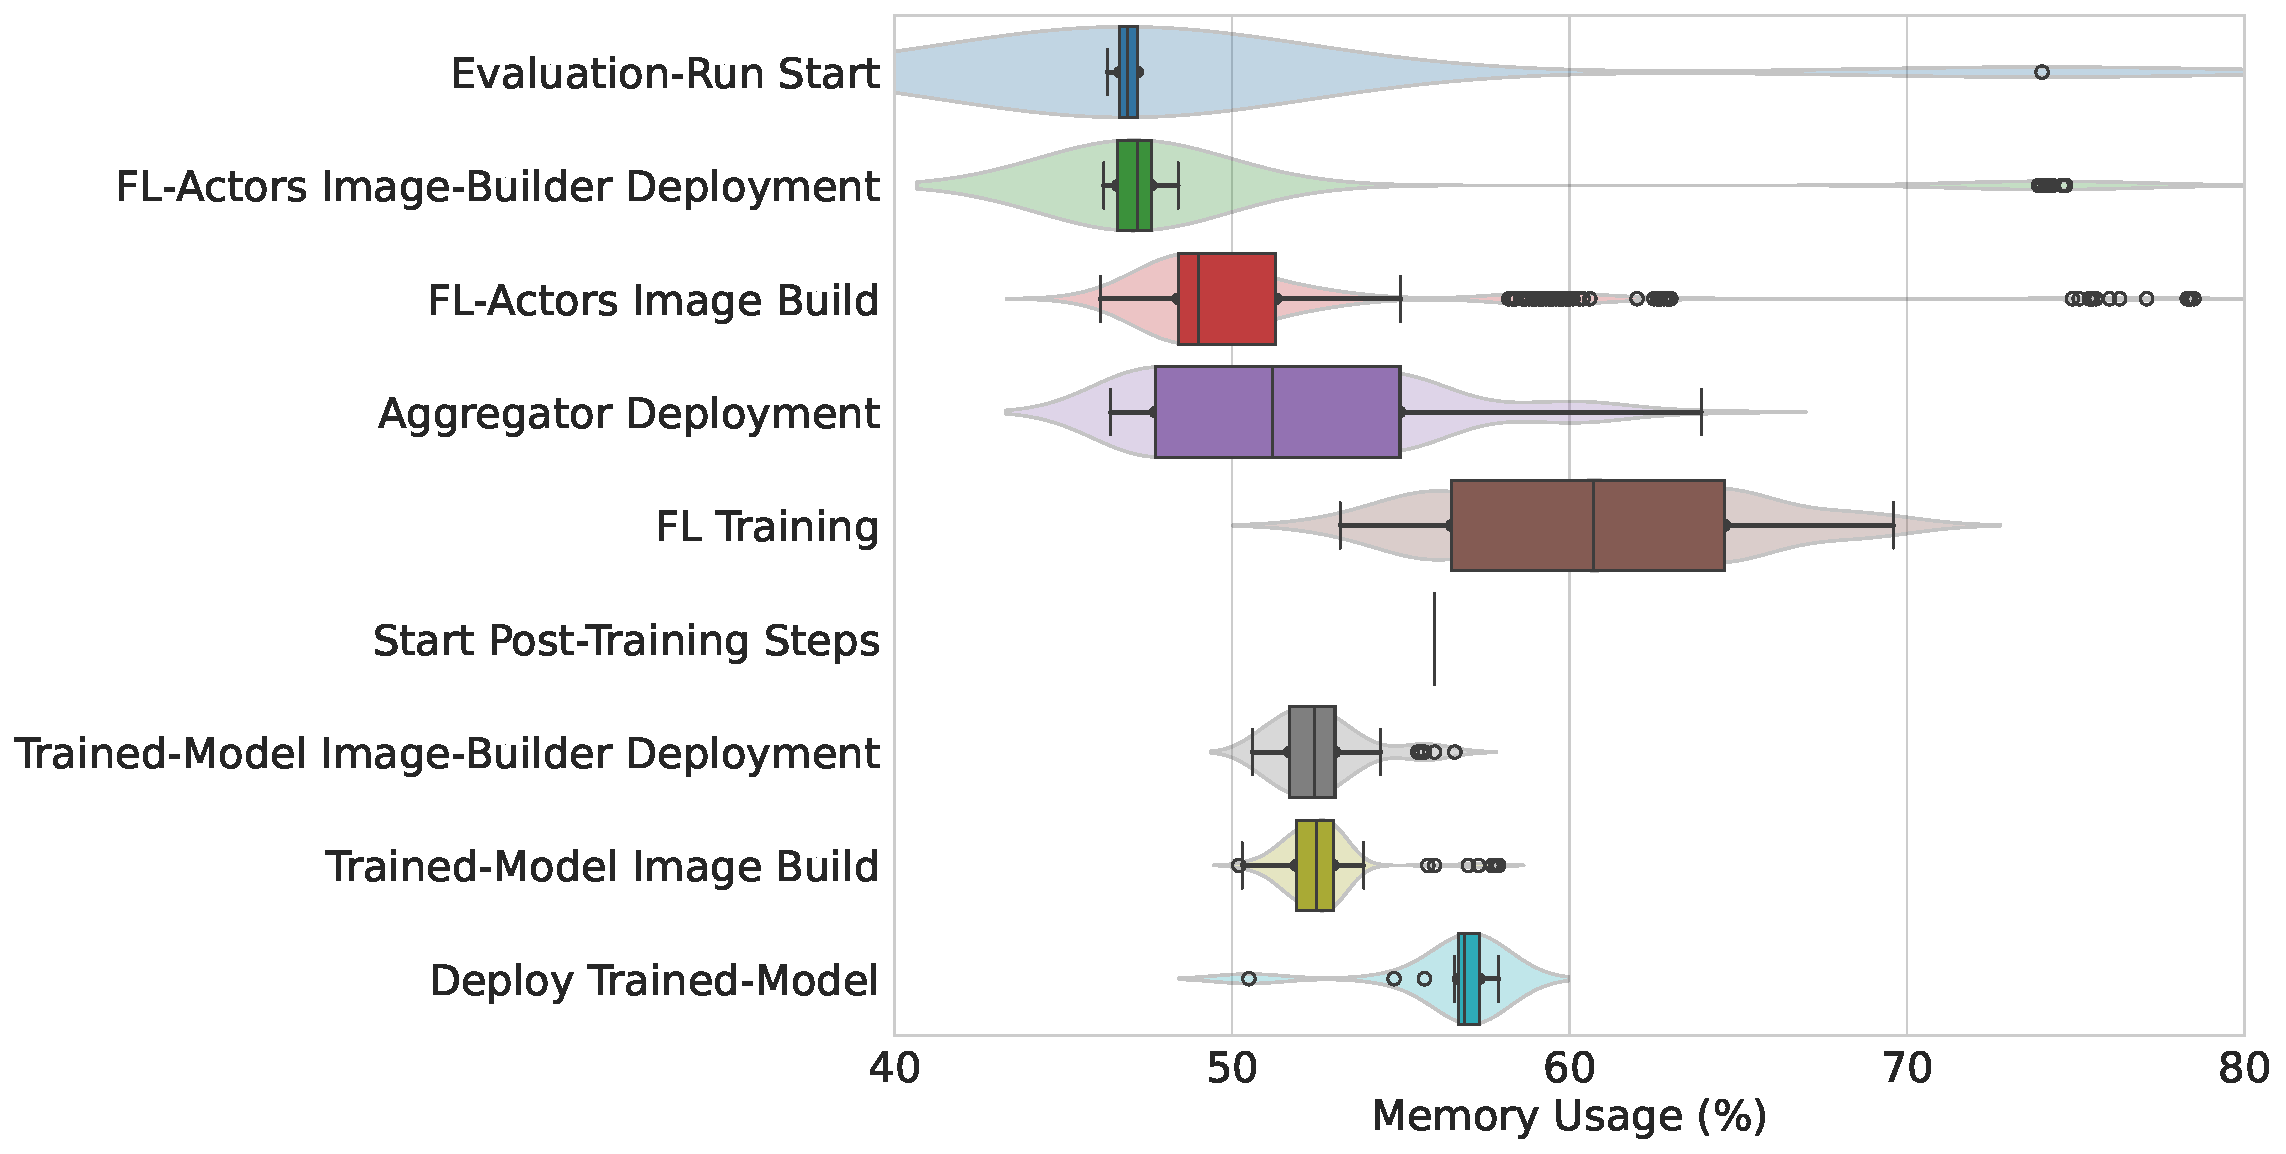
\includegraphics[width=0.85\paperwidth]{evaluations/experiment_1/mem_by_stage.pdf}
        \caption{Experiment 1: Memory Utilization by Stage}
        \label{fig:eval_1_simplest_memory_boxviolin}
    \end{adjustwidth}
\end{figure}

\pagebreak
\subsubsection{Normalization}

\begin{figure}[h]
    % \begin{adjustwidth}{-0.2\paperwidth}{-0.2\paperwidth}
        \centering
        % 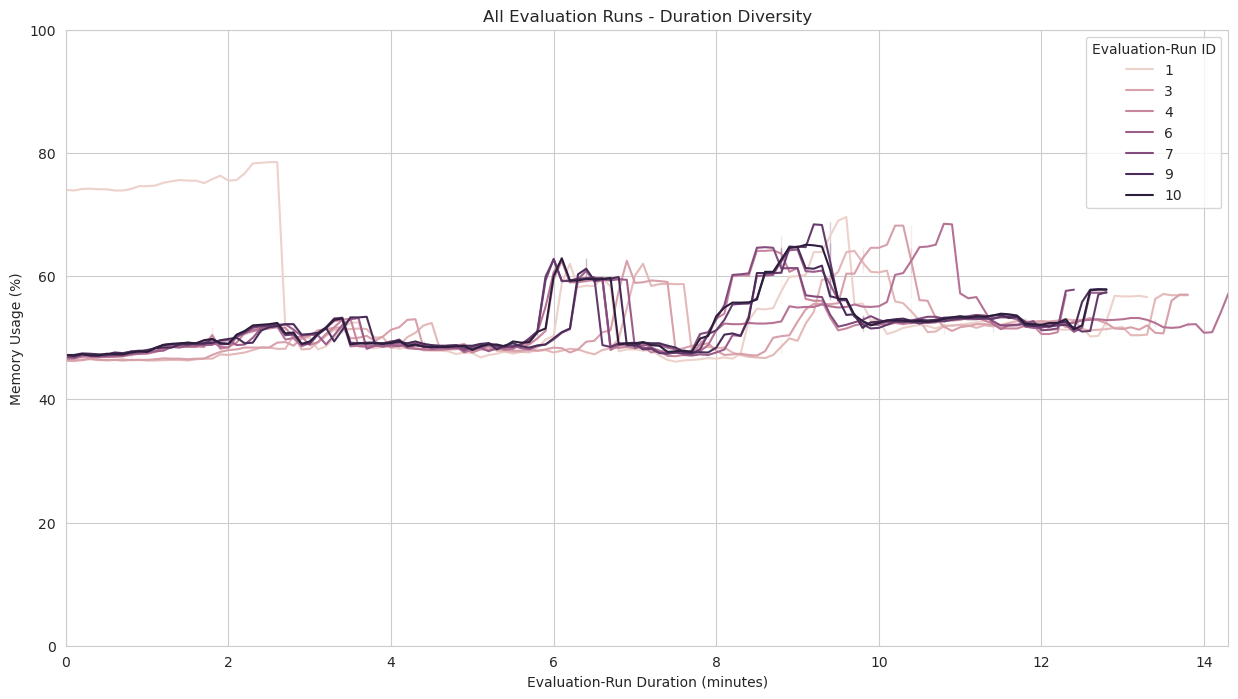
\includegraphics[width=0.99\paperwidth]{eval_1_simplest_explanation_shift.png}
        % 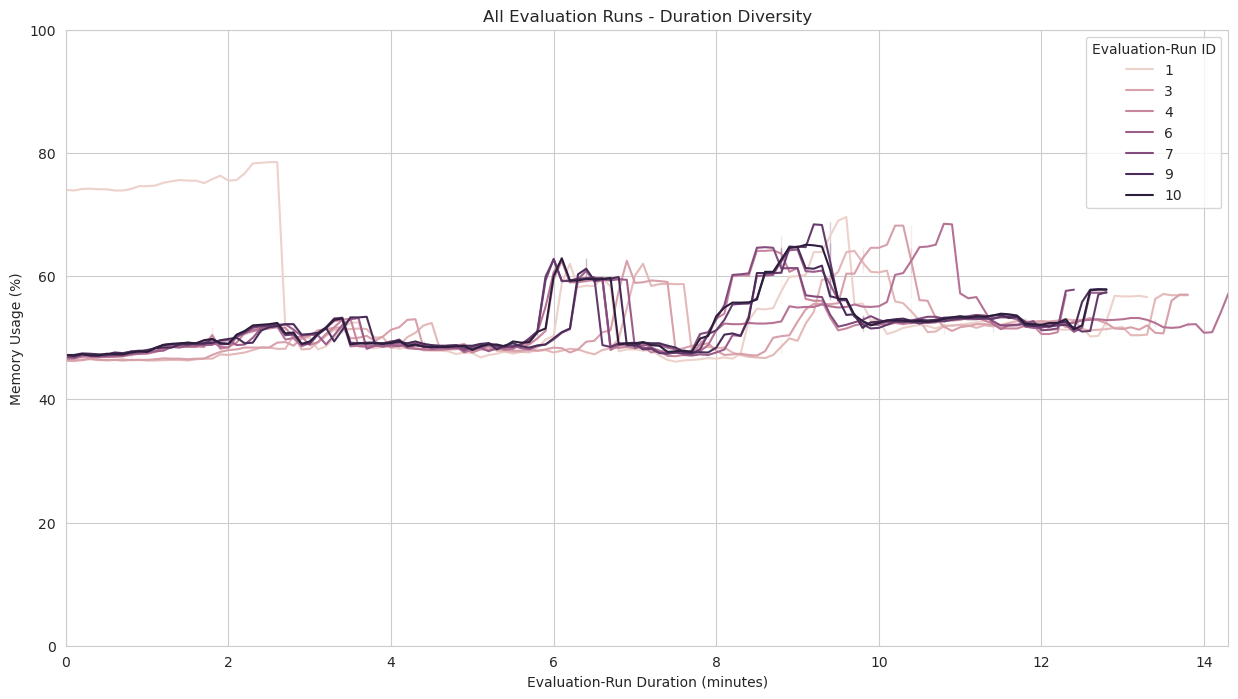
\includegraphics[width=1.0\textwidth]{eval_1_simplest_explanation_shift.png}
        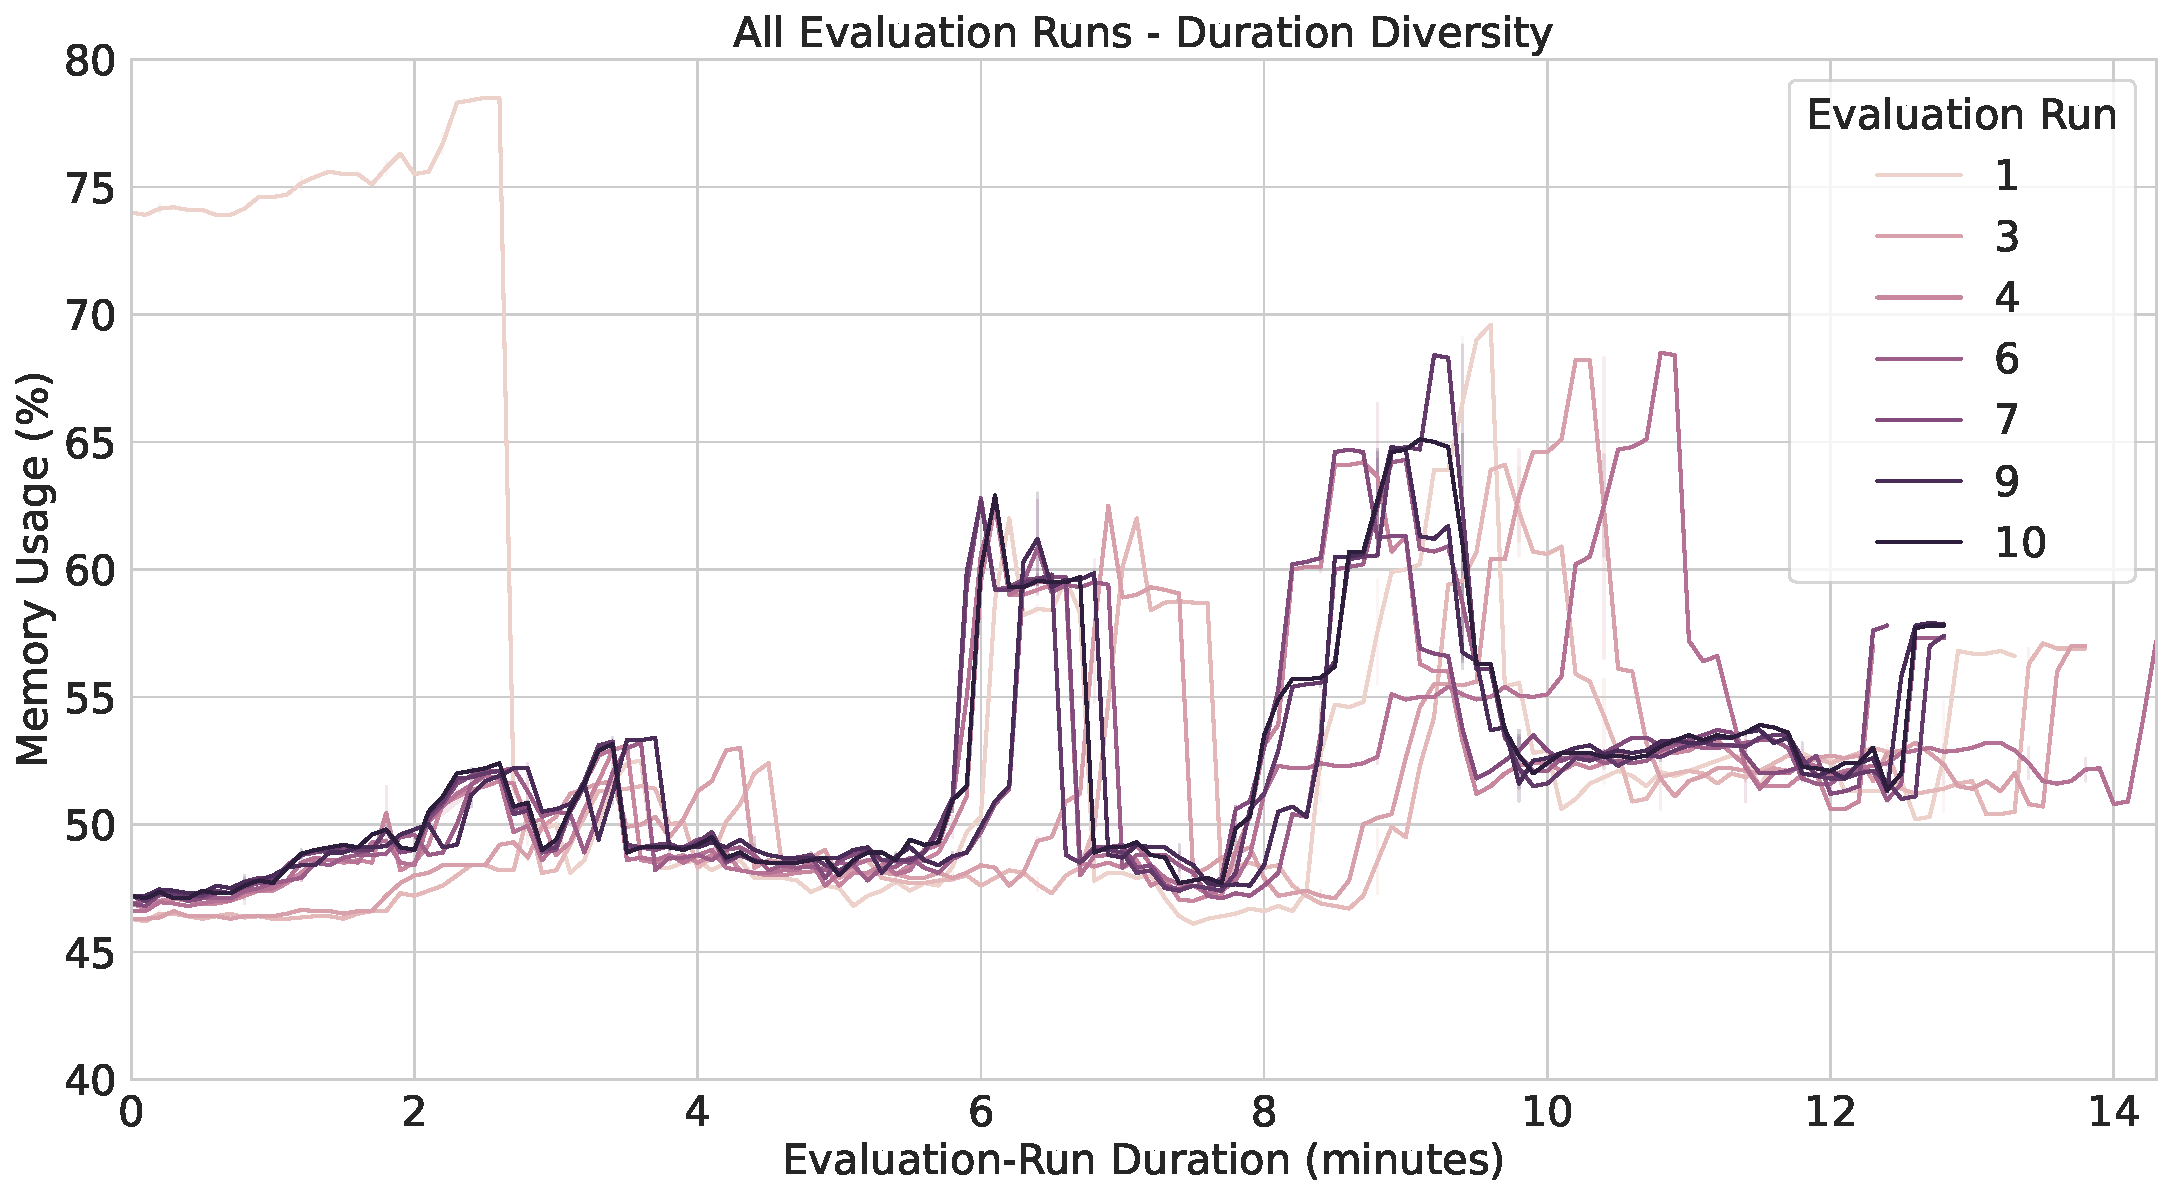
\includegraphics[width=1.0\textwidth]{evaluations/experiment_1/explanatory.pdf}
        \caption{Individual Experiment Memory Usage}
        \label{fig:eval_1_simplest_explanation_shift}
    % \end{adjustwidth}
\end{figure}

Individual evaluations range in duration.
The reasons for this can be manifold, such as different current image pull speeds due to local network conditions or remote registry loads.

Figure \ref{fig:eval_1_simplest_explanation_shift} shows the memory usage of individual evaluation rounds over time.
It is clear to see that the usage pattern is the same but shifted over time.
We normalized the average of these rounds to compare and visualize them properly.
Otherwise, stage borders become duplicated and overlapped, means and confidence intervals do not lead to meaningful outcomes, and the graphs are more confusing than helpful.

\subsubsection{Disk Space} \label{subsection:disc_space}

Graph \ref{fig:eval_1_simplest_disk_space} shows how the disk space changes over the project's lifetime.
There was a total average increase of 14 GB.
It starts with the Image-Builder-Deployment stage, where the Image-Builder image is pulled.
Many components and dependencies are downloaded and pushed to the registry on the same monolithic device during the FL actors' build process.
The jump in disk space in the aggregator (FL actors) deployment stage is because containerd needs to pull these build images.
Thus, the monolith will have the same image in the image registry and its local containerd image context.
During FL training, the disk space remains the same, which verifies that even when using FLOps with demanding lengthy training configurations and models, no disk space issues will arise due to its training process.
Disk space occasionally goes down due to the system's garbage collection, which is independent of FLOps or Oakestra.
The aggregator (FL-actors) deployment stage takes up the most space.
The trained-model image deployment stage is minimal compared to the first builder deployment because of the local containerd image storage.
Containerd pulls the builder image once and reuses it afterward.
This means that dedicated worker nodes that handle several project builds can pull these reoccurring images once and reuse them for all projects.
Especially during image-building processes, much space is freed up again due to garbage collection.

\begin{figure}[t]
    \begin{adjustwidth}{-0.2\paperwidth}{-0.2\paperwidth}
        \centering
        % 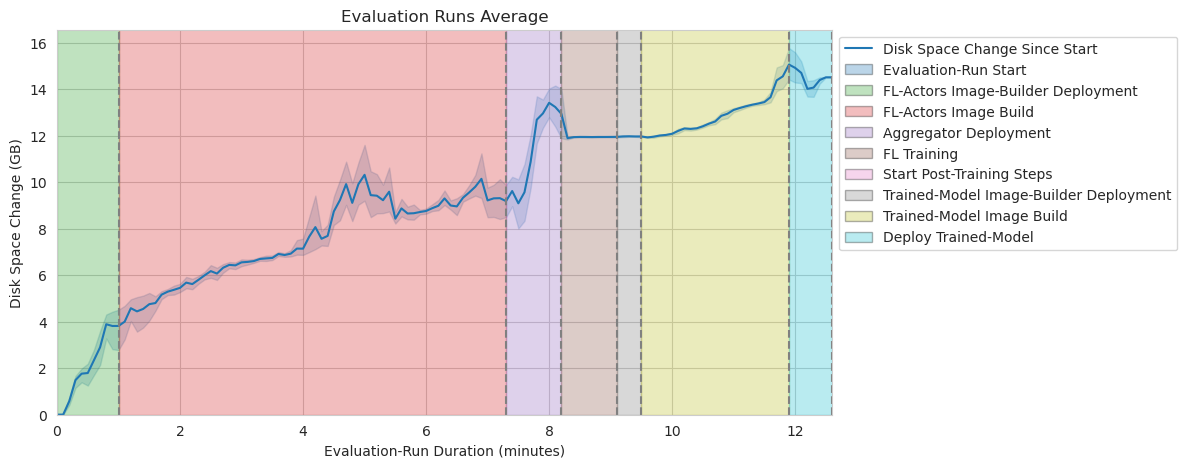
\includegraphics[width=0.99\paperwidth]{eval_1_simplest_disk_pace_linegraph.png}
        \includegraphics[width=0.99\paperwidth]{evaluations/experiment_1/disk_linear.pdf}
        \caption{Experiment 1: Disk Space Changes over Time}
        \label{fig:eval_1_simplest_disk_space}
    \end{adjustwidth}
\end{figure}

\subsubsection{Network IO}

\begin{figure}[h]
    \begin{adjustwidth}{-0.2\paperwidth}{-0.2\paperwidth}
        \centering
        % 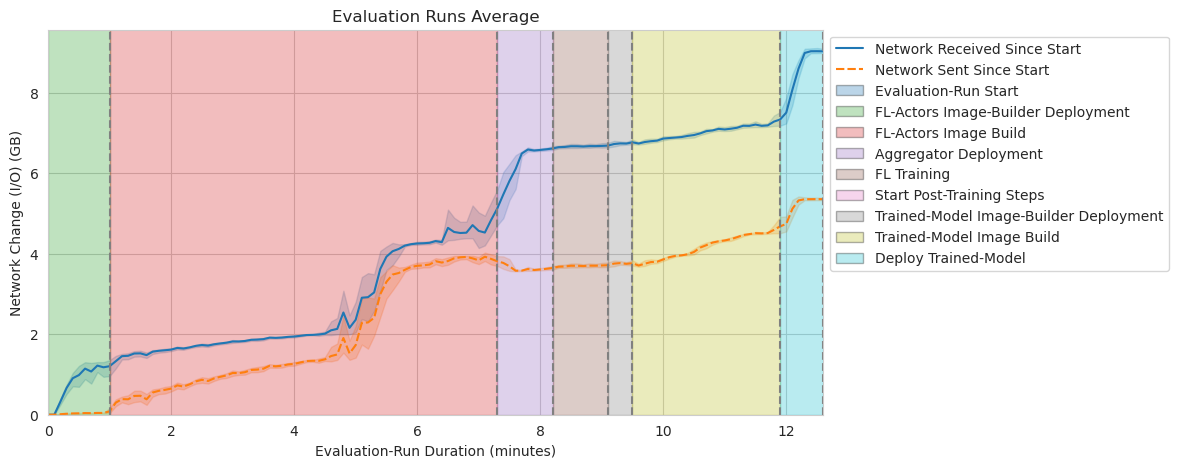
\includegraphics[width=0.99\paperwidth]{eval_1_simplest_network_linegraph.png}
        \includegraphics[width=0.99\paperwidth]{evaluations/experiment_1/net_io.pdf}
        \caption{Experiment 1: Net-IO over Time}
        \label{fig:eval_1_simplest_net_io}
    \end{adjustwidth}
\end{figure}

Figure \ref{fig:eval_1_simplest_net_io} shows the network loads received and sent over a project runtime.
The most significant increases are during built image pushes.
They occur around minute five when the base image is pushed, at the end of the FL-Actors Image Build stage phase, and when the trained-model image build stage bleeds into its deployment stage.
We omit to present further (violin-box) plots detailing net-IO because this additional information does not lead to any significant insights.

These values should be strictly increasing due to the accumulative nature of network IO counters.
This plot shows dips.
The reason for this is connected to removed containers.
The displayed lines are the sums of all received and sent traffic detectible on all network interfaces.
This includes virtual network interfaces of containers.
For example, there is a noticeable decrease between the FL-Actors image build and aggregator deployment stages.
I.e., between the moment the builder service finishes pushing its images and terminates and before these build services get deployed.
The image builder container had its own virtual network interface, which was included in the total sum and represented as a plotted line.
Once the container is removed, its virtual network interface is also deleted, and its accumulated net IO will be removed from the sum of the following system metrics scrapes.

\subsubsection{Stage Runtimes \& Training Results}
Figure \ref{fig:eval_1_simplest_stage_durations} shows each stage's average duration.
The FL training stage is relatively short because the training configuration is minimal.
The image build stages both take up the vast majority of time.
The FL-actors image build process involves more images with complex dependency resolutions.
Thus, this build stage takes over twice as long as the trained-model image build.
Figures \ref{fig:eval_1_simplest_accuracies} and \ref{fig:eval_1_simplest_loss} show the accuracies and losses of the trained models after each evaluation round.
They prove that FLOps can train ML models in a stable way.

\begin{figure}[H]
    \begin{adjustwidth}{-0.2\paperwidth}{-0.2\paperwidth}
        \centering
        % 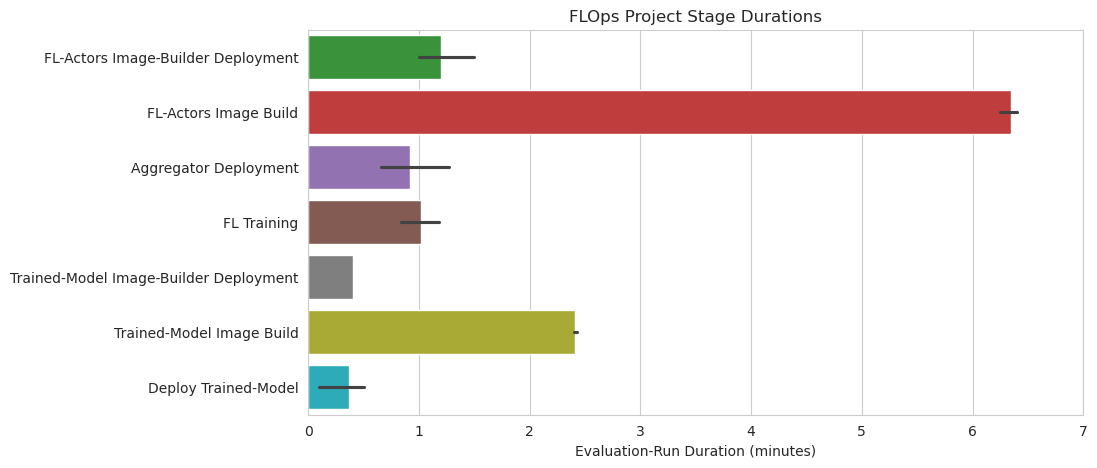
\includegraphics[width=0.80\paperwidth]{eval_1_simplest_stage_durations.png}
        \includegraphics[width=0.90\paperwidth]{evaluations/experiment_1/stage_durations.pdf}
        \caption{Experiment 1: Stage Durations}
        \label{fig:eval_1_simplest_stage_durations}
    \end{adjustwidth}
\end{figure}

\begin{figure}[H]
    \centering
    % 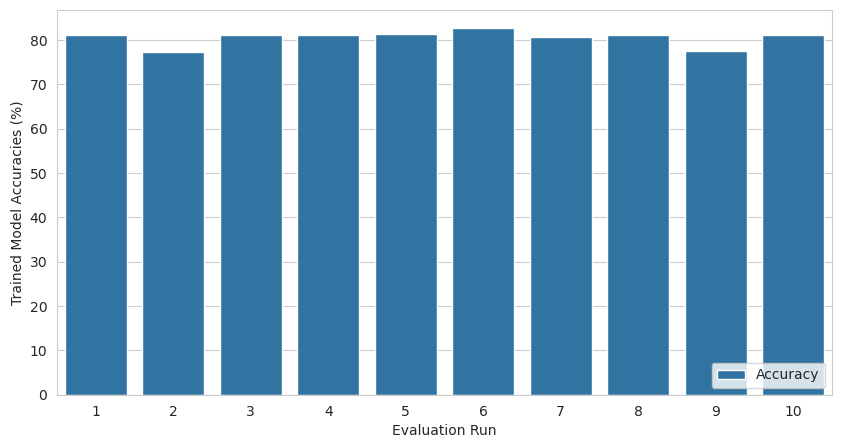
\includegraphics[width=0.90\textwidth]{eval_1_simplest_accuracy.png}
    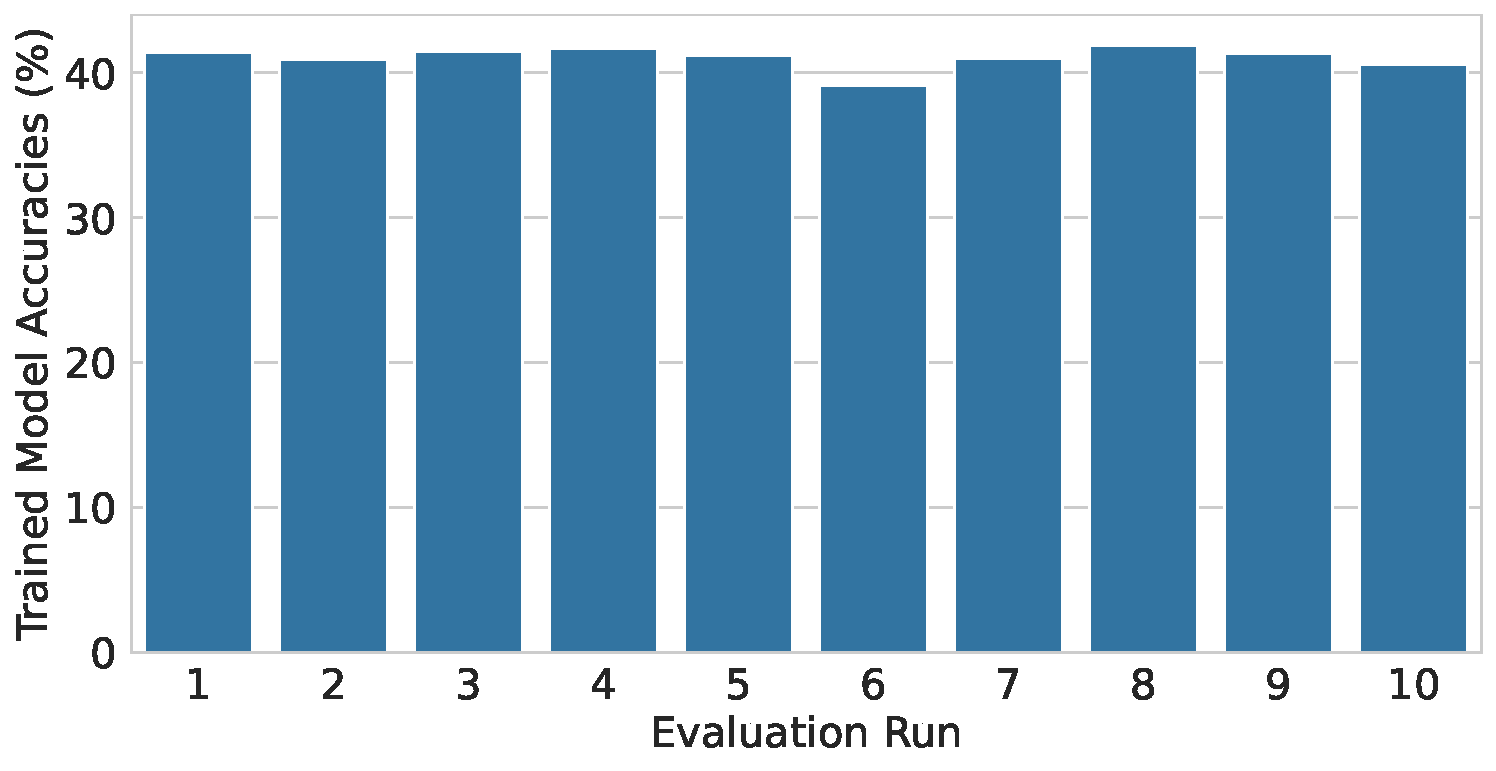
\includegraphics[width=0.90\textwidth]{evaluations/experiment_1/accuracy.pdf}
    \caption{Experiment 1: Trained Model Accuracies}
    \label{fig:eval_1_simplest_accuracies}
\end{figure}

\begin{figure}[H]
    \centering
    % 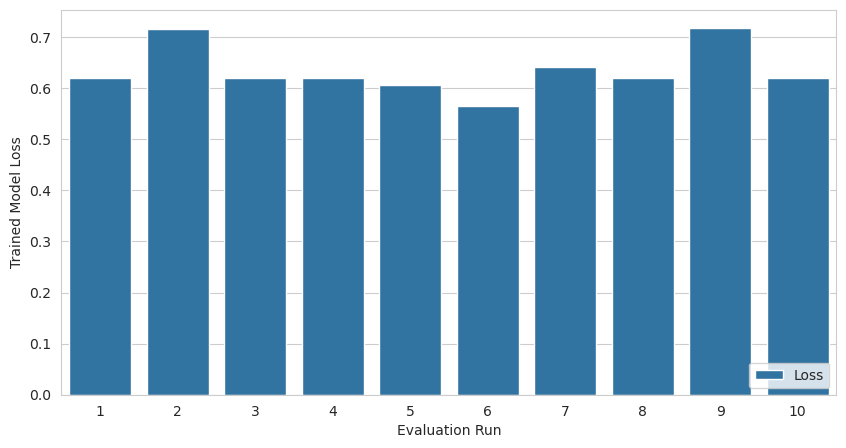
\includegraphics[width=0.90\textwidth]{eval_1_simplest_loss.png}
    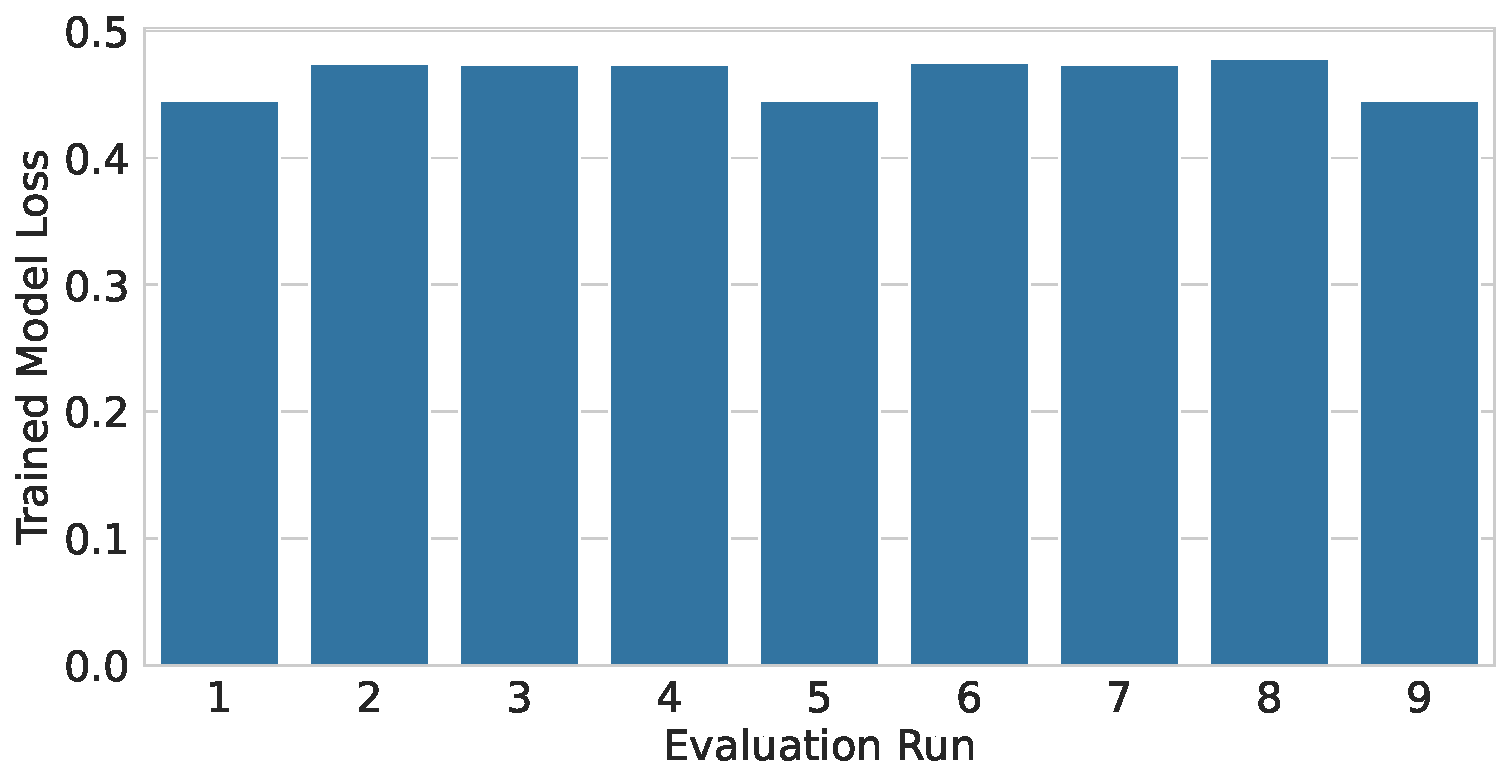
\includegraphics[width=0.90\textwidth]{evaluations/experiment_1/loss.pdf}
    \caption{Experiment 1: Trained Model Loss}
    \label{fig:eval_1_simplest_loss}
\end{figure}



\subsection{Image Builder} \label{subsection:eval_image_builder}

This subsection highlights how different variable configurations impact the total project, especially its image build times, which make up a significant part of it.

Figure \ref{fig:eval_3_cpu_and_mem} depicts the CPU and memory utilization of experiment (3).
Compared to (1), a project now only takes approximately eight minutes, and the FL-actors' build times shrunk from six to two and a half minutes.
The use of development base images leads to even greater acceleration when the underlying dependency structure of the ML repository is larger.
The base images do not apply to the trained model build because each trained model is unique.
The stage durations graph \ref{fig:eval_3_simplest_stage_durations} of experiment (3) highlights this acceleration.
All other metrics, such as net-IO, disk space, memory, or results, stay the same as in (1) because the only change is the reuse of base images.
Therefore, when people develop FLOps further, they should utilize this base-image functionality to speed up their progress.

Figure \ref{fig:eval_4_cpu_and_mem} shows the CPU and memory utilization of experiment (4).
It is immediately clear how much emulation slows down multi-platform projects compared to the base case.
A simple multi-platform project takes around 45 minutes.
The FL-actor image build stage takes 27 minutes, which is a 4.5-fold increase, and the multi-platform trained-model image build takes 13 minutes, which is a fivefold increase.
This stark difference is especially visible in Figure \ref{fig:eval_4_simplest_stage_durations}, which shows the stage durations of experiment (4).
Other metrics are also lightly affected by this change.
More disk space is needed. 
Experiment (4) uses up 17.5 GB instead of 14 GB due to the extra image layers.
This increase also influences the net-IO where (4) requires sending out 12 GB and receives 10 GB instead of (1)'s 9 GB and 5.5 GB.
In addition, the net-IO accumulated more traffic over the longer project run-time.
In conclusion, these findings prove that FLOps supports working multi-platform images.
However, this approach significantly increases build times when run on single machines instead of dedicated build machines with matching native architectures.

\begin{figure}[H]
    \begin{adjustwidth}{-0.2\paperwidth}{-0.2\paperwidth}
        \centering
        % 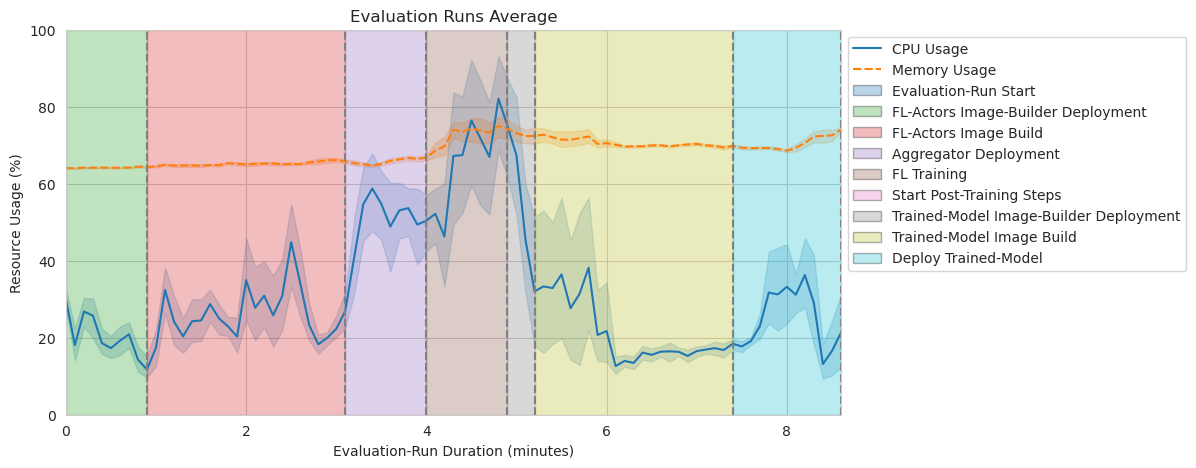
\includegraphics[width=0.90\paperwidth]{eval_3_simple_baseimages_cpu_and_mem.png}
        \includegraphics[width=0.90\paperwidth]{evaluations/experiment_3/cpu_mem.pdf}
        \caption{Experiment 3: CPU \& Memory Utilization}
        \label{fig:eval_3_cpu_and_mem}
    \end{adjustwidth}
\end{figure}

\begin{figure}[H]
    \begin{adjustwidth}{-0.2\paperwidth}{-0.2\paperwidth}
        \centering
        % 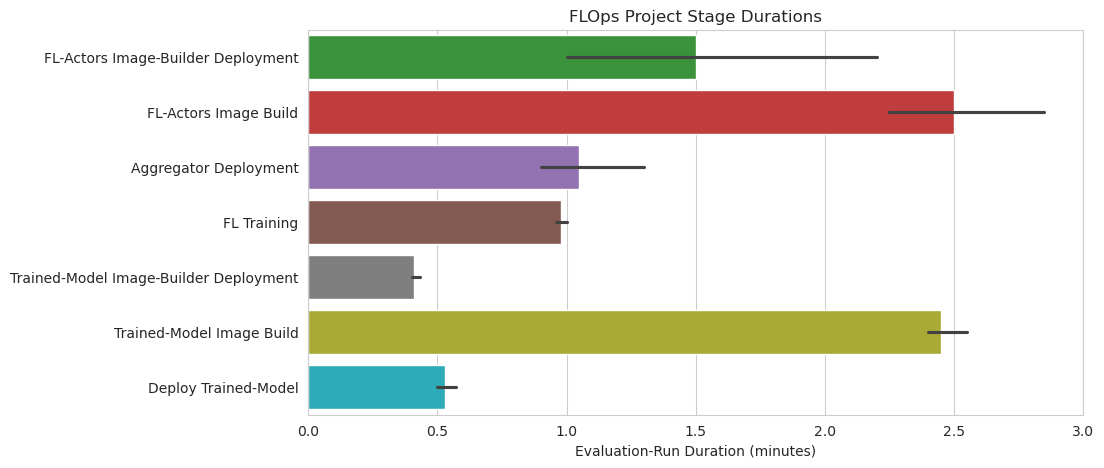
\includegraphics[width=0.95\textwidth]{eval_3_simple_baseimages_stage_durations.png}
        % \includegraphics[width=0.95\textwidth]{evaluations/experiment_3/stage_durations.pdf}
        \includegraphics[width=0.90\paperwidth]{evaluations/experiment_3/stage_durations.pdf}
        \caption{Experiment 3: Stage Durations}
        \label{fig:eval_3_simplest_stage_durations}
    \end{adjustwidth}
\end{figure}


\begin{figure}[H]
    \begin{adjustwidth}{-0.2\paperwidth}{-0.2\paperwidth}
        \centering
        % 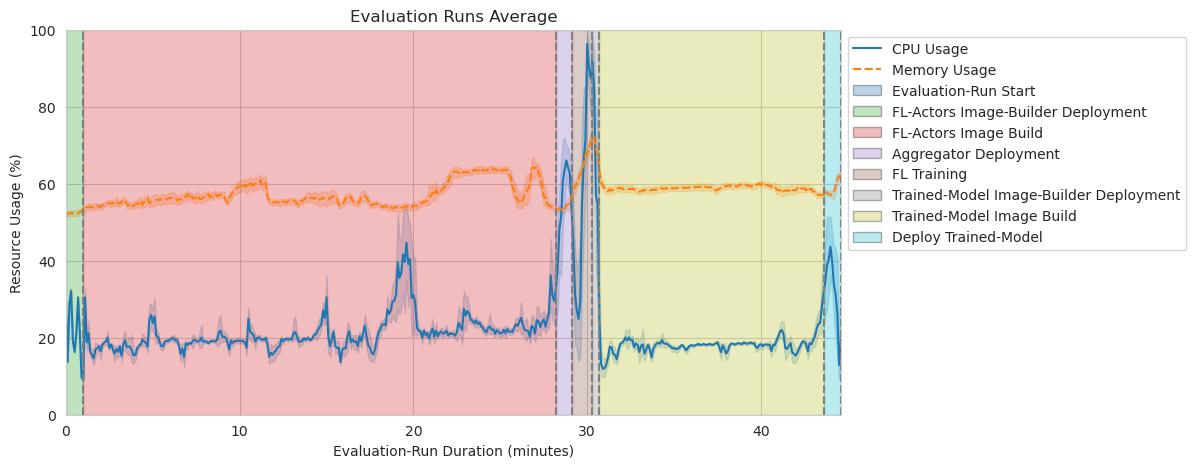
\includegraphics[width=0.90\paperwidth]{eval_4_simple_multiplatform_cpu_and_mem.png}
        \includegraphics[width=0.90\paperwidth]{evaluations/experiment_4/cpu_mem.pdf}
        \caption{Experiment 4: CPU \& Memory Utilization}
        \label{fig:eval_4_cpu_and_mem}
    \end{adjustwidth}
\end{figure}

\begin{figure}[H]
    \begin{adjustwidth}{-0.2\paperwidth}{-0.2\paperwidth}
        \centering
        % 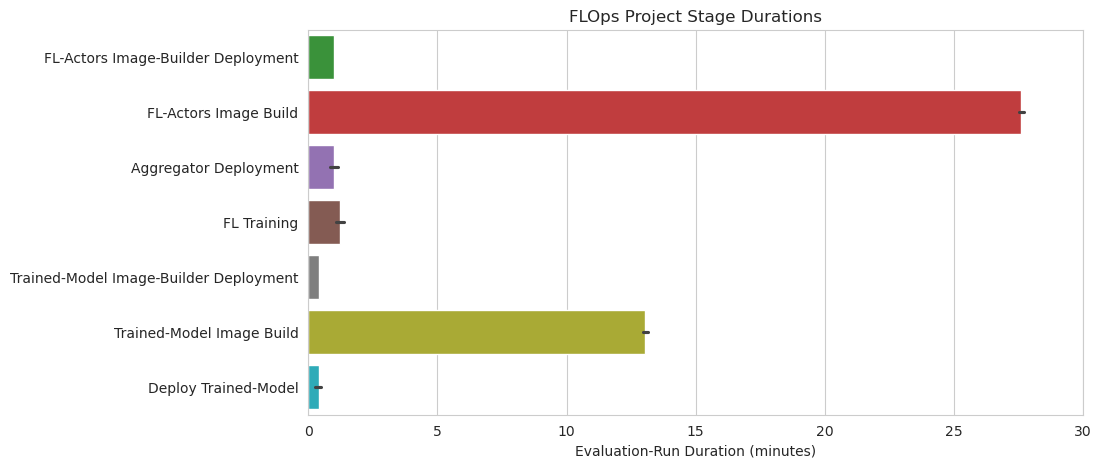
\includegraphics[width=0.95\textwidth]{eval_4_simple_multiplatform_stage_durations.png}
        \includegraphics[width=0.90\paperwidth]{evaluations/experiment_4/stage_durations.pdf}
        \caption{Experiment 4: Stage Durations}
        \label{fig:eval_4_simplest_stage_durations}
    \end{adjustwidth}
\end{figure}


\subsection{Fundamentally Different Projects} \label{subsection:eval_diff_projects}

\subsubsection{Longer Training Rounds with more Learners}

Figure \ref{fig:eval_2_cpu_mem} shows the CPU and memory utilization of experiment (2).
Because this project configuration uses more learners and training rounds, it is logical that the FL training stage will last longer.
Note that this larger example is still relatively small compared to ML/FL training periods that take multiple hours or days to complete.
The CPU utilization during training is less spread than for (1) and concentrates in the high 90-100\% range.
Memory shows a similar shift from the low 60s to the low 70s.
The disk space and net-IO stay similar to (1).
The resulting accuracies are now all in the mid-80s instead of below 80\%.
Extended training periods lead to better results in this case.

\begin{figure}[t]
    \begin{adjustwidth}{-0.2\paperwidth}{-0.2\paperwidth}
        \centering
        % 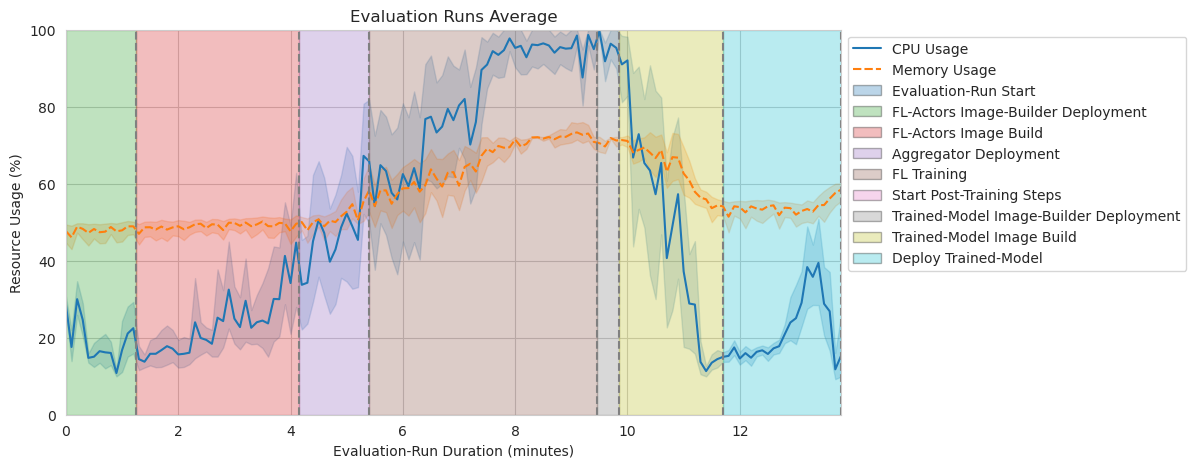
\includegraphics[width=0.85\paperwidth]{eval_2_simple_large_cpu_and_mem.png}
        \includegraphics[width=0.90\paperwidth]{evaluations/experiment_2/cpu_mem.pdf}
        \caption{Experiment 2: CPU \& Memory}
        \label{fig:eval_2_cpu_mem}
    \end{adjustwidth}
\end{figure}

\subsubsection{Different ML Repository, Framework, and Dataset}
Figure \ref{fig:eval_5_cpu_mem} shows the CPU and memory utilization of experiment (5).
The first noticeable difference to (1) is the almost threefold project duration, mainly due to build times.
Pytorch is a more heavy-weight ML library than Scikit-learn.
Thus, configuring its larger dependencies takes longer.
(5)'s CPU behavior is similar to (1).
The FL training in (5) requires less memory (mid 50s) than in (1) (low 60s).

Figure \ref{fig:eval_5_disk_space} shows the remarkable influence of the chosen ML framework and its dependencies for FLOps.
Compared to the relatively lightweight Sklearn base-case example with a total used disk space increase of 14 GB, this simple Pytorch example takes up approximately 35 GB in the end.
During build times when dependencies are pulled, the peak extra disk space utilization reaches 60 GB.
These heavy dependencies are also visible in the network IO in Figure \ref{fig:eval_5_net_io}.
The garbage collection is strongly present and visible in this case.
The tiny number of learners and training rounds lead to a small accuracy of 40\% of the final models.

\begin{figure}[p]
    \begin{adjustwidth}{-0.2\paperwidth}{-0.2\paperwidth}
        \centering
        % 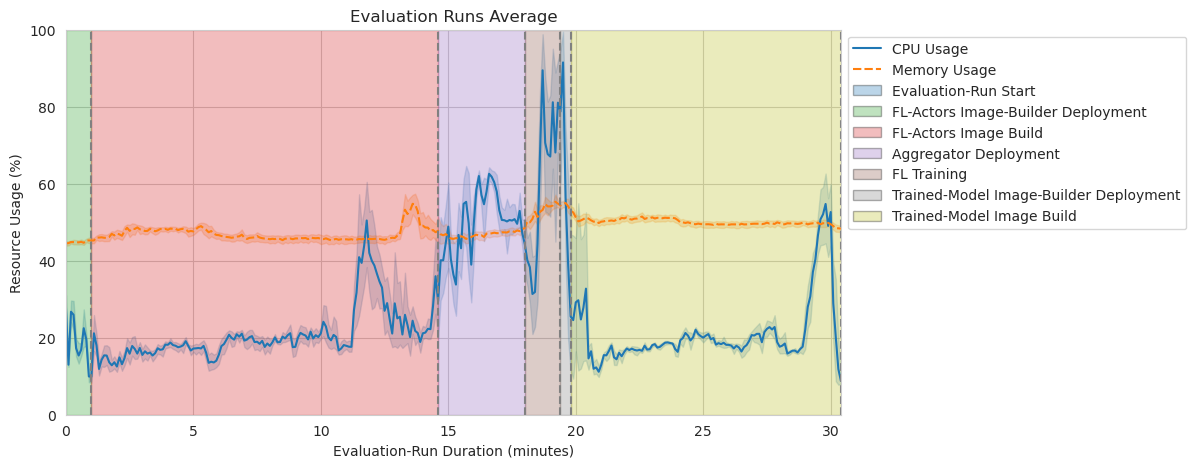
\includegraphics[width=0.80\paperwidth]{eval_5_simple_pytorch_cpu_and_mem.png}
        \includegraphics[width=0.85\paperwidth]{evaluations/experiment_5/cpu_mem.pdf}
        \caption{Experiment 5: CPU \& Memory}
        \label{fig:eval_5_cpu_mem}
    \end{adjustwidth}

    \begin{adjustwidth}{-0.2\paperwidth}{-0.2\paperwidth}
        \centering
        % 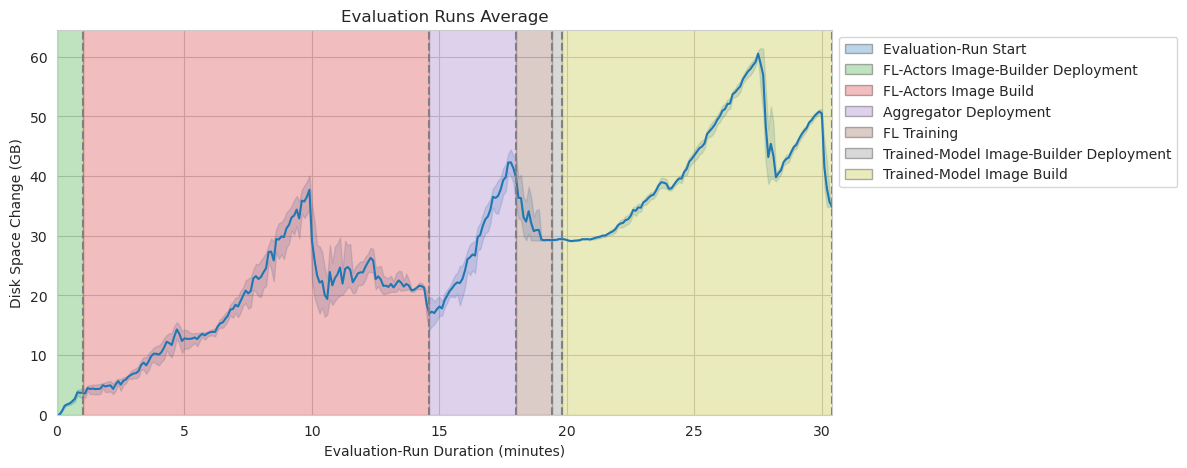
\includegraphics[width=0.80\paperwidth]{eval_5_simple_pytorch_disk_space.png}
        \includegraphics[width=0.85\paperwidth]{evaluations/experiment_5/disk_linear.pdf}
        \caption{Experiment 5: Disk Space}
        \label{fig:eval_5_disk_space}
    \end{adjustwidth}

    \begin{adjustwidth}{-0.2\paperwidth}{-0.2\paperwidth}
        \centering
        % 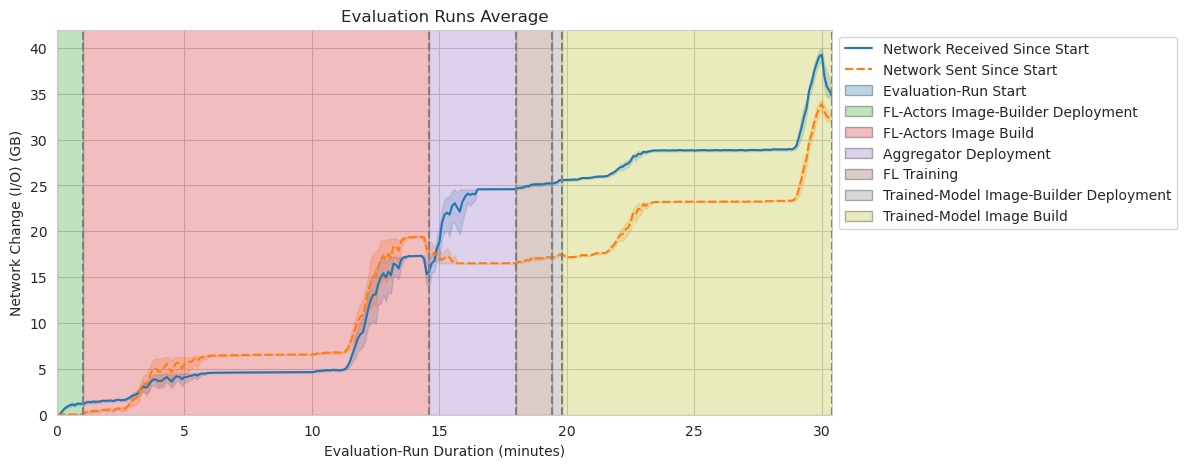
\includegraphics[width=0.80\paperwidth]{eval_5_simple_pytorch_net_io.png}
        \includegraphics[width=0.85\paperwidth]{evaluations/experiment_5/net_io.pdf}
        \caption{Experiment 5: Network IO}
        \label{fig:eval_5_net_io}
    \end{adjustwidth}
\end{figure}

These experiments prove that FLOps can handle different FL training configurations using various ML frameworks, repositories, and datasets.
They also unveil that using popular classic ML libraries might be unrealistic for resource-constrained edge devices.
Thus, libraries that are dedicated to restricted devices should be analyzed and tried out as future work.

% \pagebreak


\subsection{Multi-cluster \& HFL} \label{subsection:eval_multicluster_hfl}

\subsubsection{Classic FL on the Multi-Cluster Setup}

Before analyzing how real HFL performs on multiple clusters, we need to verify that the second setup is capable of classic FL and compare it to the monolith setup.
Observing the aggregated sum of metrics from all three devices leads to flat and less insightful plots.
For this reason, the following graphs will depict the metrics by device.
Figure \ref{fig:eval_7_cpu} shows the CPU utilization of the cluster setup during experiment (7).
It depicts how the control plane root device only manages components but does not perform any heavy operations as intended.
Its CPU utilization is constantly at a very low level.
The orchestrator selected and deployed the image builder service on cluster B.
That is why it is the only busy device during the initial image build phase.
Notably, this scheduling decision seems to be deterministic.
The orchestrator independently selected Cluster B for every single run.
Once FL actor deployment and training start, CPU utilization gets distributed among both cluster nodes.
Figure \ref{fig:eval_7_mem} shows the memory utilization of the devices.
The memory stays stable when no workloads are performed on a device, which is the case for the root at all times and for cluster-A while cluster-B is building the images. 
The reason why the root device has a higher memory usage then the two clusters is because the root hosts the control plane.
This includes Oakestra's root orchestrator and all FLOps management components.

Figure \ref{fig:eval_7_disk_space} shows the increase in disk space for the devices.
It shows how cluster-B's disk space is increasing during the build process due to the dependencies and layers that are pulled and build.
There is a drop after the build process finishes, and the builder service is undeployed.
In the middle of the build process, cluster B pushes the built base image to the root that hosts the image registry.
Cluster-B pushes the FL-actor images without a significant increase because the common base layers are reused.
The disk space of cluster-A only starts increasing when the FL actors are deployed on it.
Figures \ref{fig:eval_7_net_received} and \ref{fig:eval_7_net_send} show the received and sent network changes on the devices, matching the disk space changes.
The FLOps stages seen in Figure \ref{fig:eval_7_stage_durations} of experiment (7) do not show any remarkable outliers and resemble the base case.
The only difference is that the project and its stages take longer due to the weaker hardware.
Project stages on our multi-cluster setup take approximately 0.67 to 7.5 (average 2.88) times longer than on the monolith setup.
Because stages have different durations and weights the overall runtime of a project only increased by approximately 1.67 times.
The final training results are equivalent to (1).



\begin{figure}[p]

    \begin{adjustwidth}{-0.2\paperwidth}{-0.2\paperwidth}
        \centering
        % 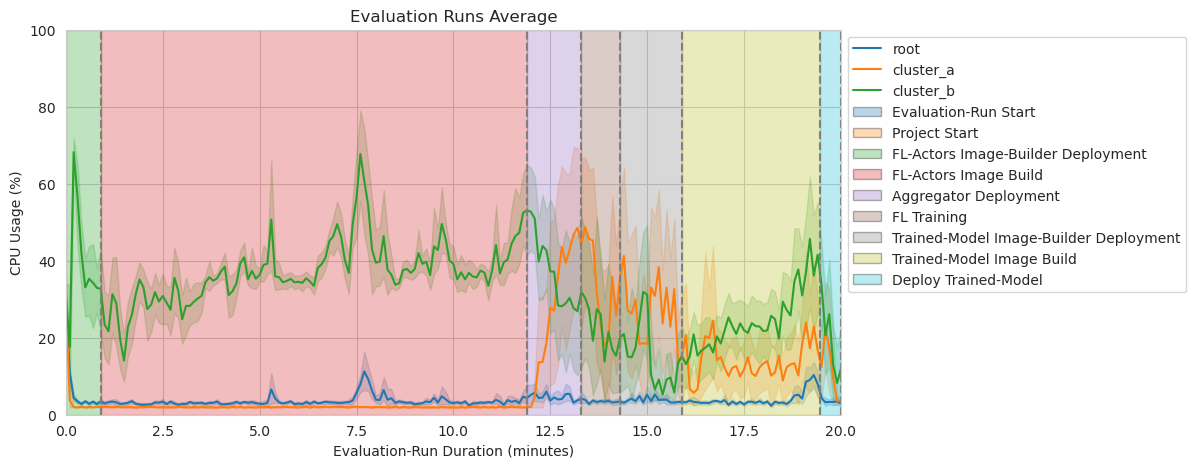
\includegraphics[width=0.95\paperwidth]{evaluations/multicluster_hfl/eval_9_7_simple_multicluster_cpu_split.png}
        \includegraphics[width=0.85\paperwidth]{evaluations/experiment_7/cpu.pdf}
        \caption{Experiment 7: CPU Utilization}
        \label{fig:eval_7_cpu}
    \end{adjustwidth}

    \begin{adjustwidth}{-0.2\paperwidth}{-0.2\paperwidth}
        \centering
        \includegraphics[width=0.85\paperwidth]{evaluations/experiment_7/mem.pdf}
        \caption{Experiment 7: Memory Utilization}
        \label{fig:eval_7_mem}
    \end{adjustwidth}

    \begin{adjustwidth}{-0.2\paperwidth}{-0.2\paperwidth}
        \centering
        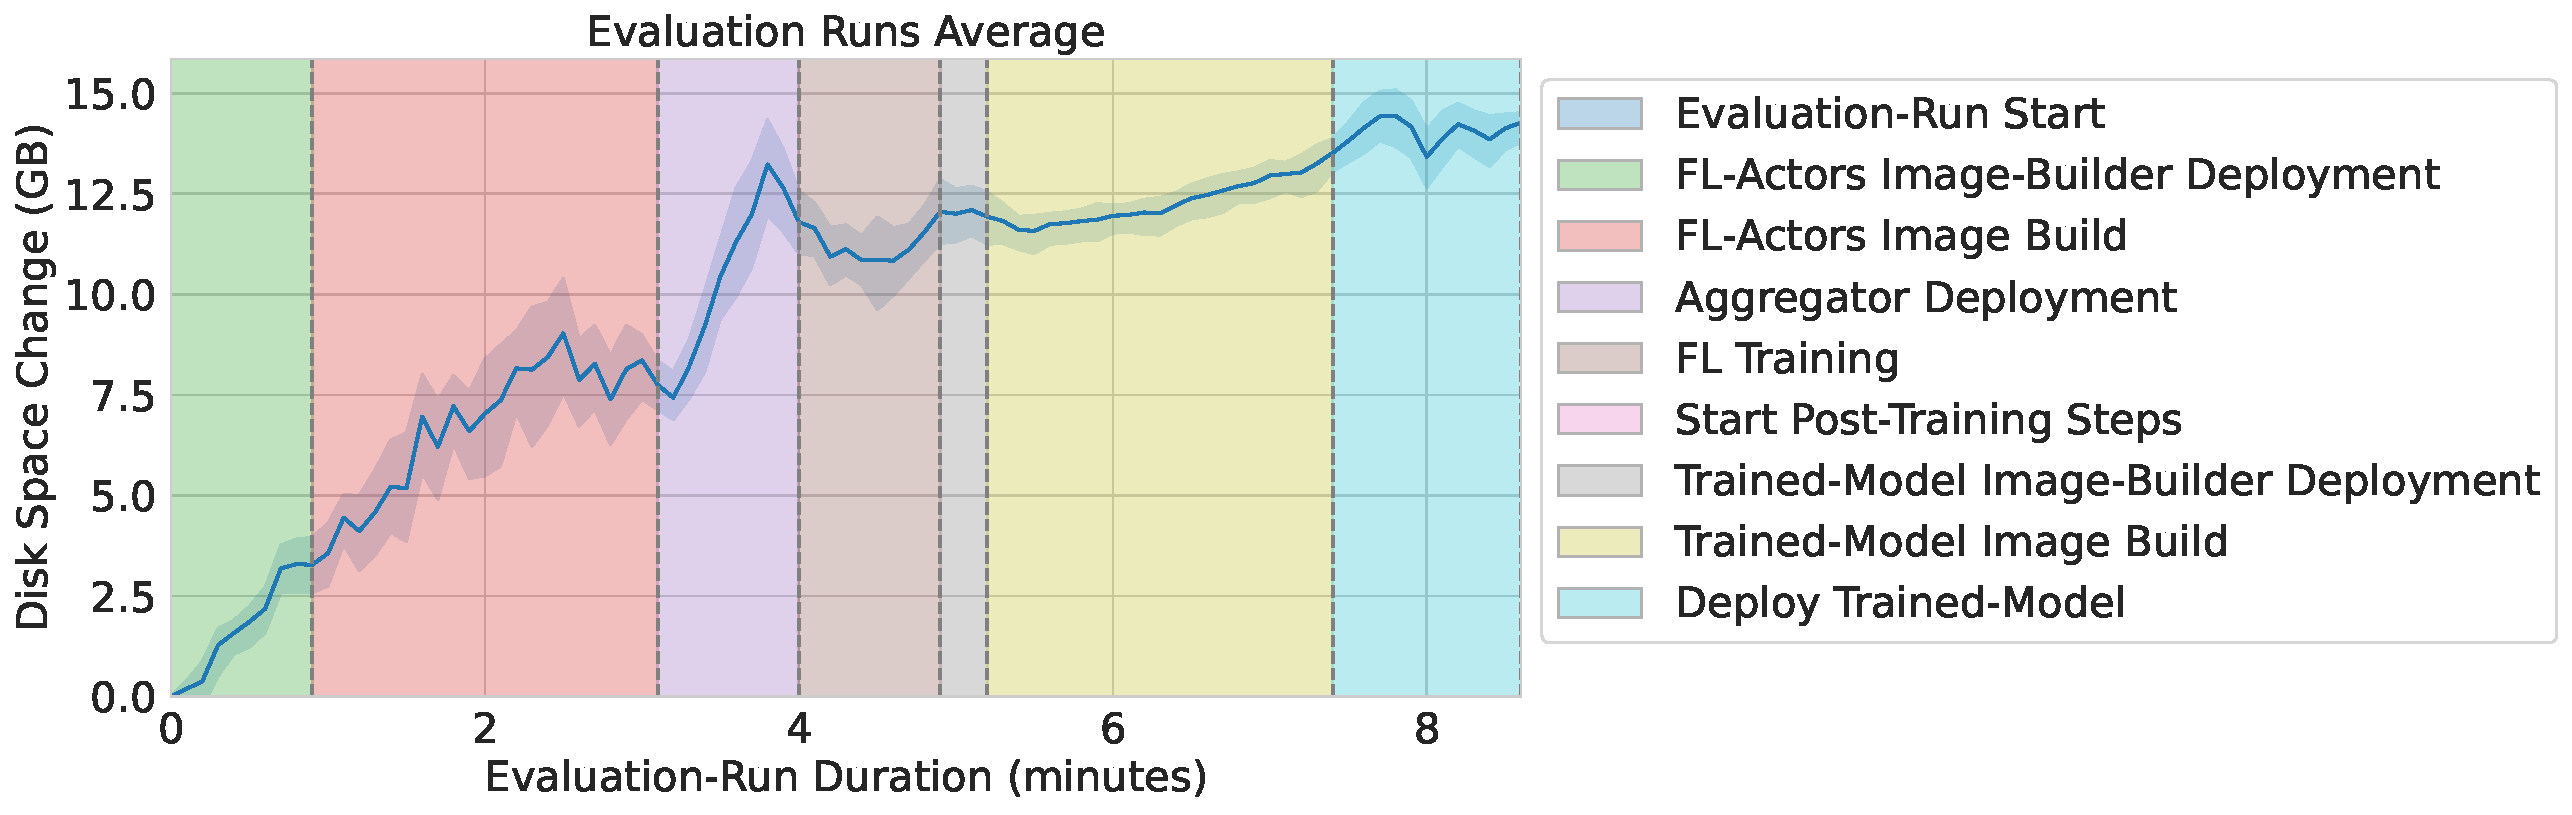
\includegraphics[width=0.85\paperwidth]{evaluations/experiment_7/disk.pdf}
        \caption{Experiment 7: Disk Space}
        \label{fig:eval_7_disk_space}
    \end{adjustwidth}
\end{figure}

\begin{figure}[p]
    \begin{adjustwidth}{-0.2\paperwidth}{-0.2\paperwidth}
        \centering
        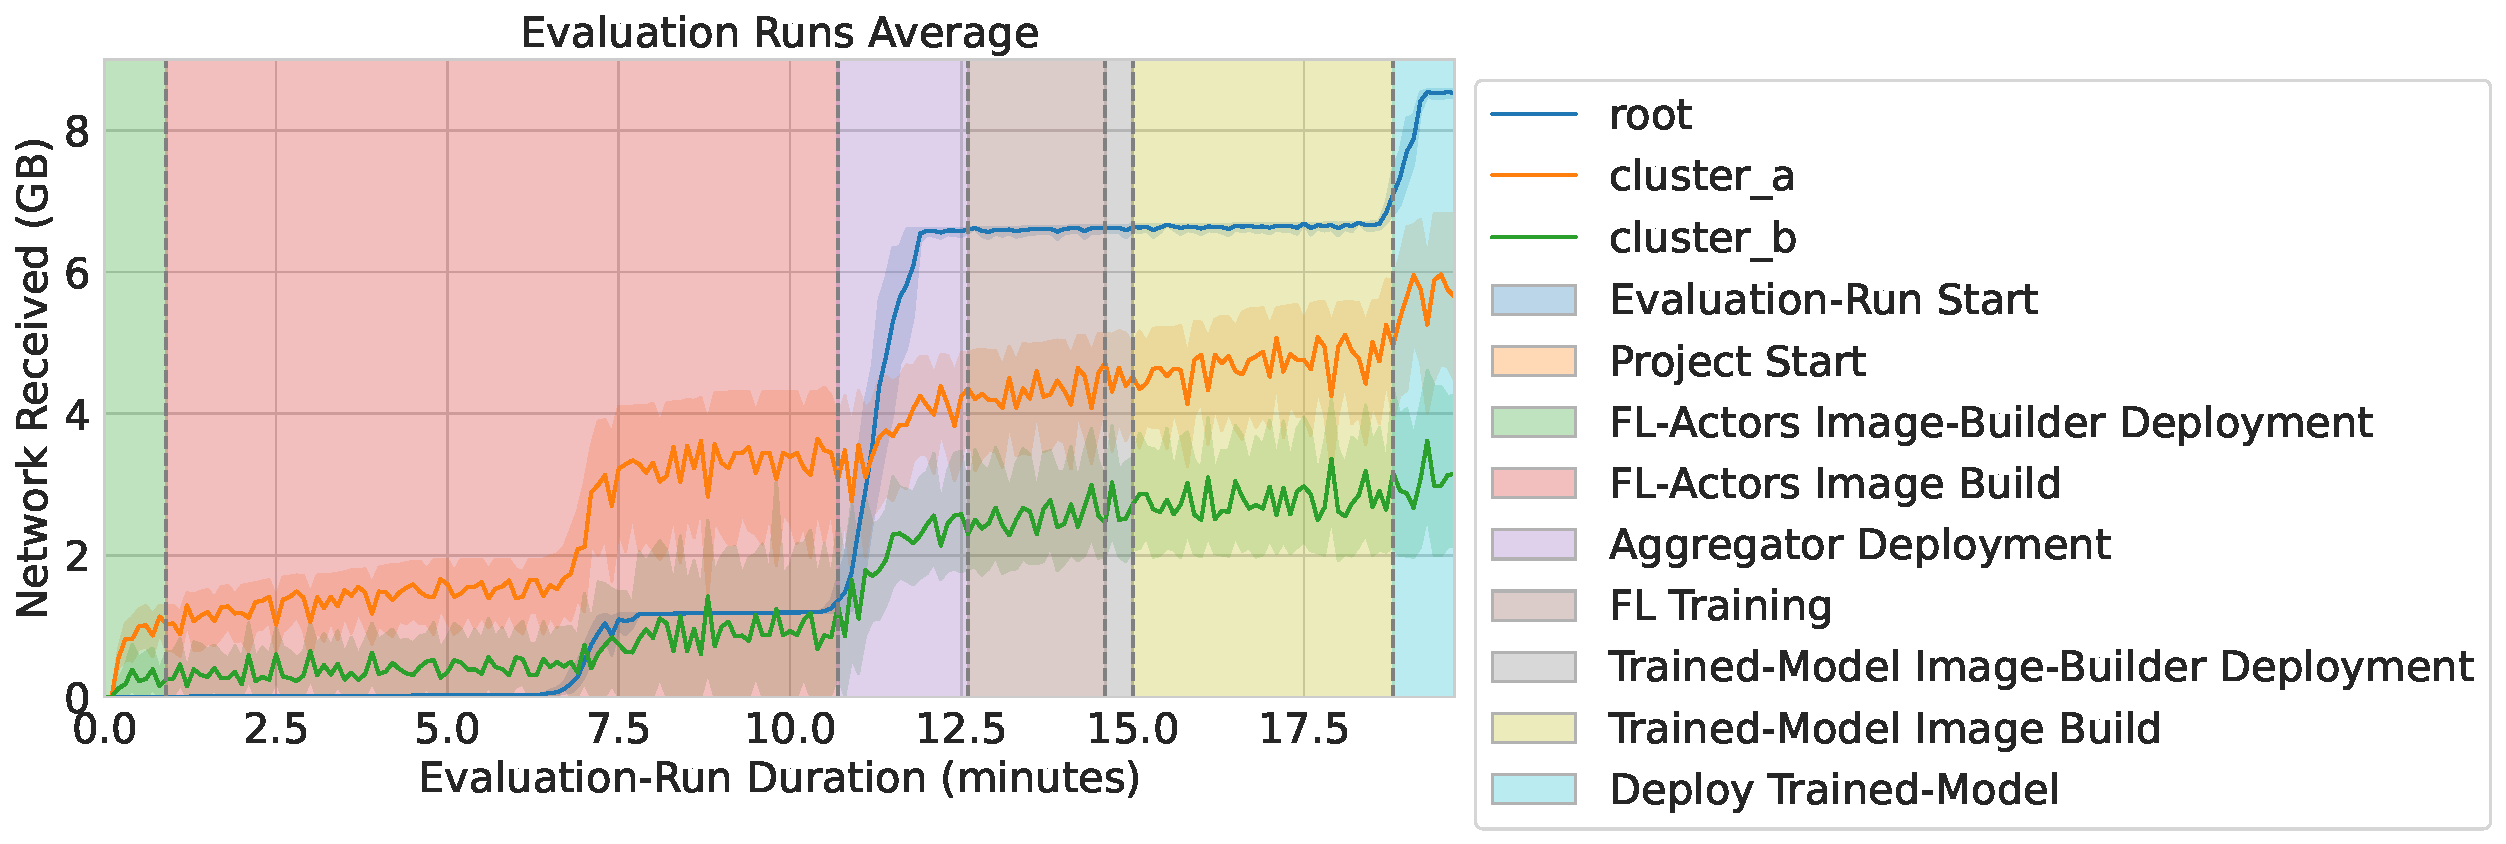
\includegraphics[width=0.83\paperwidth]{evaluations/experiment_7/net_received.pdf}
        \caption{Experiment 7: Received Network}
        \label{fig:eval_7_net_received}
    \end{adjustwidth}

    \begin{adjustwidth}{-0.2\paperwidth}{-0.2\paperwidth}
        \centering
        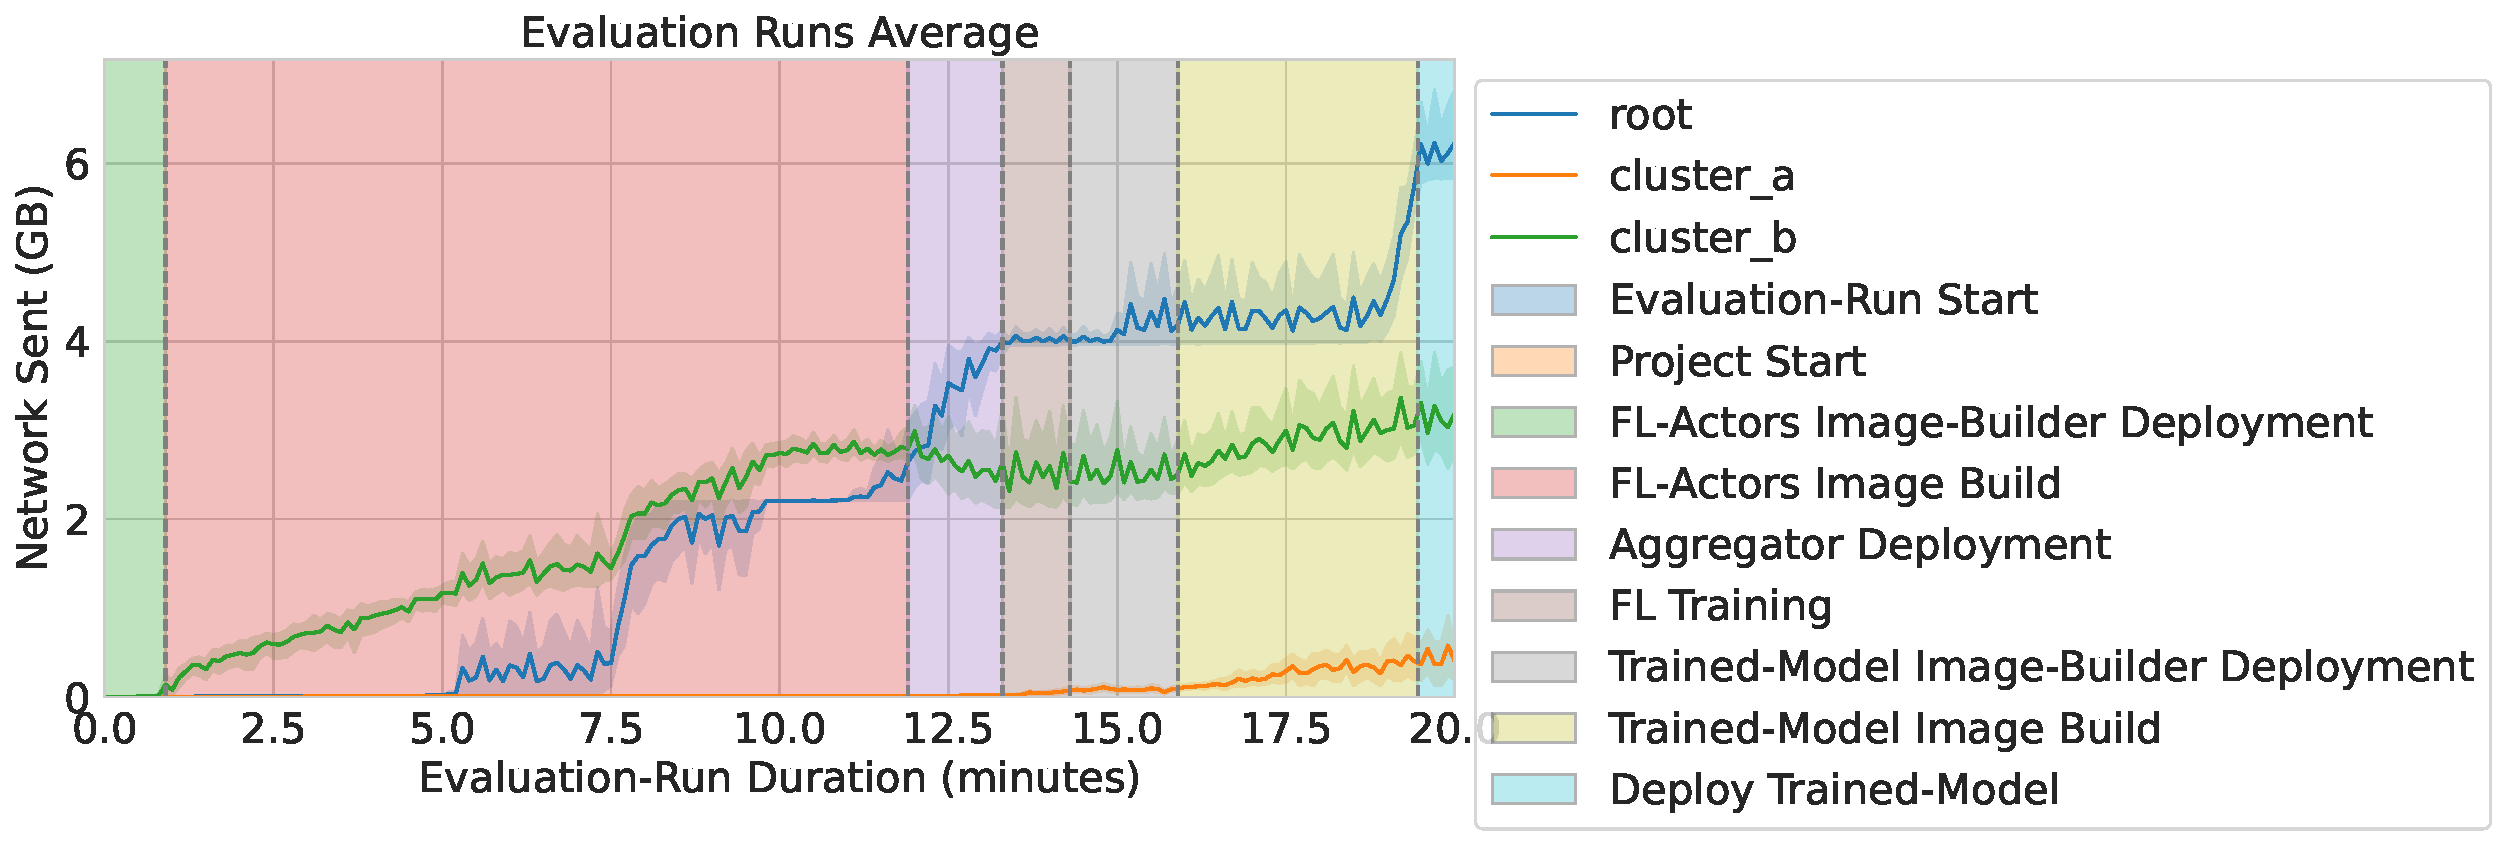
\includegraphics[width=0.83\paperwidth]{evaluations/experiment_7/net_sent.pdf}
        \caption{Experiment 7: Send Network}
        \label{fig:eval_7_net_send}
    \end{adjustwidth}

    \begin{adjustwidth}{-0.2\paperwidth}{-0.2\paperwidth}
        \centering
        \includegraphics[width=0.80\paperwidth]{evaluations/experiment_7/stage_durations.pdf}
        \caption{Experiment 7: Stage Durations}
        \label{fig:eval_7_stage_durations}
    \end{adjustwidth}
\end{figure}

\pagebreak

\subsubsection{Minimal HFL base-case on a monolith Cluster}

\begin{figure}[H]
    \begin{adjustwidth}{-0.2\paperwidth}{-0.2\paperwidth}
        \centering
        \includegraphics[width=0.95\paperwidth]{evaluations/experiment_6/cpu_mem.pdf}
        \caption{Experiment 6: Monolith HFL CPU \& Memory}
        \label{fig:eval_6_cpu_mem}
    \end{adjustwidth}
\end{figure}

Figure \ref{fig:eval_6_cpu_mem} shows the CPU and memory utilization of experiment (6).
Its purpose is to be a minimal HFL base-case that only uses a single cluster.
In additon, this experiment proofs that FLOps' custom clustered HFL solution works.
Compared to (1) the project duration is a bit longer due to the longer training stage.
Every other metric stays similar to (1).
This includes the stage durations, disk space, net IO, and training results.
CPU and memory utilization are slightly increased in the deployment and training stages because of more FL actors.


\subsubsection{HFL on the Multi-Clustered Setup}

Figure \ref{fig:eval_8_cpu} shows the CPU utilization of the multi-cluster setup devices during HFL.
The image build seems to be no longer handled by a single cluster but is more distributed among both.
In (7), learners were randomly deployed on clustered.
In (8), the figure clearly shows that the CPU is utilized more and distributed more equally among the clusters.
This is the case because each cluster gets its own cluster aggregator and set of learners.
This more homogeneous utilization also applies to memory, as Figure \ref{fig:eval_8_mem} shows.
All other metrics show a similar change from (7) to (8) as from (1) to (6).
This includes disk space, net IO, stage durations (Figure \ref{fig:eval_8_stage_durations}), and training results.
These findings prove that FLOps can perform clustered HFL on distributed multi-cluster devices.


\begin{figure}[p]
    \begin{adjustwidth}{-0.2\paperwidth}{-0.2\paperwidth}
        \centering
        \includegraphics[width=0.85\paperwidth]{evaluations/experiment_8/cpu.pdf}
        \caption{Experiment 8: Multi-Cluster HFL CPU Utilization}
        \label{fig:eval_8_cpu}
    \end{adjustwidth}

    \begin{adjustwidth}{-0.2\paperwidth}{-0.2\paperwidth}
        \centering
        \includegraphics[width=0.85\paperwidth]{evaluations/experiment_8/mem.pdf}
        \caption{Experiment 8: Multi-Cluster HFL Memory Utilization}
        \label{fig:eval_8_mem}
    \end{adjustwidth}

    \begin{adjustwidth}{-0.2\paperwidth}{-0.2\paperwidth}
        \centering
        \includegraphics[width=0.80\paperwidth]{evaluations/experiment_8/stage_durations.pdf}
        \caption{Experiment 8: Stage Durations}
        \label{fig:eval_8_stage_durations}
    \end{adjustwidth}
\end{figure}